%!TEX root = ./thesis.tex

% \chapter{Template}\label{chapter:kapitellabel} %%%%%%%%%%%%%%%%%%%%%%%%%%%%
% \section{Test}
% \subsection{Sub Test}
% Itaque earum rerum hic tenetur a sapiente delectus, ut aut reiciendis voluptatibus maiores alias consequatur aut perferendis doloribus asperiores repellat\cite{aho:dragonbook}. See Table ~\ref{table:speedup1} and ~\ref{table:speedup1} and \ref{figure:helloworld}.

% \begin{table}[!th]
%   \renewcommand{\arraystretch}{1.3}
%   \caption{Speed-Up Table I}\label{table:speedup1}
%   \vspace{4mm} % hack
%   \centering
%     \begin{tabular}{|l||r|r|r|}
%       \hline
%       program            & basline   & algorithm 1  & alogrithm 2\\
%       \hline
%       \hline
%       {\tt simple}       &  30 sec   &  20 sec      &  18 sec     \\
%       \hline
%       {\tt hello world}  &  43 sec   &  27 sec      &  28 sec     \\
%       \hline
%     \end{tabular}
% \end{table}

% \begin{table}[!th]
%   \renewcommand{\arraystretch}{1.3}
%   \caption{Speed-Up Table II}\label{table:speedup2}
%   \vspace{4mm} % hack
%   \centering
%     \begin{tabular}{|l||r|r|r|}
%       \hline
%       program            & basline   & algorithm 1  & alogrithm 2\\
%       \hline
%       \hline
%       {\tt simple}       &  30 sec   &  20 sec      &  18 sec     \\
%       \hline
%       {\tt hello world}  &  43 sec   &  27 sec      &  28 sec     \\
%       \hline
%     \end{tabular}
% \end{table}
% Lorem ipsum dolor sit amet, consectetur adipiscing elit, sed do eiusmod tempor incididunt ut labore et dolore magna aliqua. Ut enim ad minim veniam, quis nostrud exercitation ulla hghgh hhghg mco laboris nisi ut aliquip ex ea commodo consequat. Duis aute irure dolor in reprehenderit in voluptate velit esse cillum dolore eu fugiat nulla pariatur. Excepteur sint occaecat cupidatat non proident, sunt in culpa qui officia deserunt mollit anim id est laborum

% \begin{figure}[!ht]
% \centering
% \sourcecode{main.cpp}
% \caption{Hello World Program}\label{figure:helloworld}
% \end{figure}
% Lorem ipsum dolor sit amet, consectetur adipiscing elit, sed do eiusmod tempor incididunt ut labore et dolore magna aliqua. Ut enim ad minim veniam, quis nostrud exercitation ullamco laboris nisi ut aliquip ex ea commodo consequat. Duis aute irure dolor in reprehenderit in voluptate velit esse cillum dolore eu fugiat nulla pariatur. Excepteur sint occaecat cupidatat non proident, sunt in culpa qui officia deserunt mollit anim id est laborum

% Lorem ipsum dolor sit amet, consectetur adipiscing elit, sed do eiusmod tempor incididunt ut labore et dolore magna aliqua. Ut enim ad minim veniam, quis nostrud exercitation ullamco laboris nisi ut aliquip ex ea commodo consequat. Duis aute irure dolor in reprehenderit in voluptate velit esse cillum dolore eu fugiat nulla pariatur. Excepteur sint occaecat cupidatat non proident, sunt in culpa qui officia deserunt mollit anim id est laborum~\cite{GorillaArm}

% \begin{figure}[!ht] % see https://en.wikibooks.org/wiki/LaTeX/Floats,_Figures_and_Captions for placement parameters
%   \centering
%   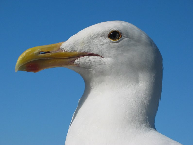
\includegraphics[width=0.5\textwidth]{images/gull.png}
%   \caption{A picture of a gull.}
% \end{figure}

% Lorem ipsum dolor sit amet, consectetur adipiscing elit, sed do eiusmod tempor incididunt ut labore et dolore magna aliqua. Ut enim ad minim veniam, quis nostrud exercitation ullamco laboris nisi ut aliquip ex ea commodo consequat. Duis aute irure dolor in reprehenderit in voluptate velit esse cillum dolore eu fugiat nulla pariatur. Excepteur sint occaecat cupidatat non proident, sunt in culpa qui officia deserunt mollit anim id est laborum

% Lorem ipsum dolor sit amet, consectetur adipiscing elit, sed do eiusmod tempor incididunt ut labore et dolore magna aliqua. Ut enim ad minim veniam, quis nostrud exercitation ullamco laboris nisi ut aliquip ex ea commodo consequat. Duis aute irure dolor in reprehenderit in voluptate velit esse cillum dolore eu fugiat nulla pariatur. Excepteur sint occaecat cupidatat non proident, sunt in culpa qui officia deserunt mollit anim id est laborum

% Lorem ipsum dolor sit amet, consectetur adipiscing elit, sed do eiusmod tempor incididunt ut labore et dolore magna aliqua. Ut enim ad minim veniam, quis nostrud exercitation ullamco laboris nisi ut aliquip ex ea commodo consequat.
% \begin{figure}[H]
%   \centering
%   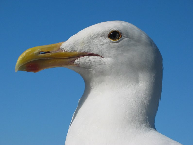
\includegraphics[width=0.5\textwidth]{images/gull.png}
%   \caption{A picture of a gull.}
% \end{figure}
% Duis aute irure dolor in reprehenderit in voluptate velit esse cillum dolore eu fugiat nulla pariatur. Excepteur sint occaecat cupidatat non proident, sunt in culpa qui officia deserunt mollit anim id est laborum

% Lorem ipsum dolor sit amet, consectetur adipiscing elit, sed do eiusmod tempor incididunt ut labore et dolore magna aliqua. Ut enim ad minim veniam, quis nostrud exercitation ullamco laboris nisi ut aliquip ex ea commodo consequat. Duis aute irure dolor in reprehenderit in voluptate velit esse cillum dolore eu fugiat nulla pariatur. Excepteur sint occaecat cupidatat non proident, sunt in culpa qui officia deserunt mollit anim id est laborum

\chapter{Einführung}\label{chapter:intro}

Zweibeiniges Gehen bietet als Fortbewegungsart durch virtuelle Umgebungen viele Vorteile gegenüber alternativen Fortbewegungsarten.[

    %TODO:Quelle
    ]
beschreibt beispielsweise, ein höheres Präsensgefühl der Nutzer:innen.[
    %TODO: Quelle

]
zeigt dass weniger Motion sickness entsteht wenn sich die Nutzer:innen durch die virtuelle Welt bewegen indem sie gehen.
[
    %TODO: quelle

]
erklärt, dass beim Gehen mehr Sinne stimuliert werden als bei künstlichen Alternativen, wie zum Beispiel der Joystick Steuerung. Tiefensensibilität (Propriozeption) und Gleichgewichtssinn (vestibuläre Wahrnehmung) signalisieren, dass er gerade wirklich geht, während diese Information bei alternativen Fortbewegungsart allein vom visuellen Sinn übermittelt wird.
Leider bring das reale gehen (real walking nach[
    %TODO: quelle

]
) auch den großen Nachteil mit sich, dass es in der Regel auf einen einzelnen Raum (den Trackingspace) beschränkt ist.

Dies entsteht zum einen, durch räumlich limitierte Erfassung (auf Englisch: tracking) der Position und Rotation des Headsets und der Controller bei einigen Technologien (zum Beispiel den Modellen der \textquote{HTC VIVE}-Produktreihe
%TODO:quelle%
), zum anderen durch die Raumgröße der meisten VR-Setups.

Zwar gibt es dazu auch Ausnahmen, ( siehe z.B.[
    %TODO: quelle microsoft studie
]
), jedoch sind diese dann mit großem Aufwand verbunden und nicht für jede Endnutzer:in umzusetzen.

\section{Redirections Techniques} %oder lieber deutsch???
%sind impossible spaces überhaupt redirected walking?
Eine Herangehensweise dieses Problem zu Umgehen sind so genannte \textquote{Redirection Techniques} (besser bekannt als Redirected Walking, diese Begriffe werden oft austauschbar verwendet (nach [
    %quelle steinicke übersicht paper

])). Dies ist ein Sammelbegriff für Techniken bei denen die Nutzer:in mit Manipulationen der Fortbewegungsart durch den Trackingspace navigiert wird.
%  Dabei wird die Illusion aufrecht erhalten sie würde sich unverändert, frei bewegen.
So lässt sich die Nutzer:in von den äußeren Begrenzungen des Trackingspaces fern halten, und die virtuell begehbare Fläche vergrößern.
Im folgenden werde ich nun zwei dieser Techniken genauer vorstellen.

\subsection{Rotationgains}
%TODO: quelle steinicke zusammenfassung der techniken
Rotationgains werden Kopfrotationen hinzugefügt sodass sich die virtuelle Kamera leicht schneller oder langsamer dreht als der reale
Kopf mit dem VR-Headset. Kopfrotationen lassen sich mit der Schreibweise
$$ R_{real} := (pitch_{real}, yaw_{real}, roll_{real}) $$
darstellen, wobei pitch, yaw und roll
die Eulerschen Winkel der Kopfrotation darstellen. Der Rotationgain wird dann als Quotient des virtuellen Winkels und des realen Winkels definiert also:
$$ gR := \frac{R_{virtual}}{R_{real}} $$
Für alle 3 Winkel kann ein Rotationgain angewandt werden.
Dieses Anwenden funktioniert indem der Rotationgain $gR$ mit dem Winkel der realen Kopfrotation $\alpha$ multipliziert wird also:
$$ gR * \alpha $$
Da für jeden Winkel der Kopfrotation ein Rotationgain definiert werden kann werden Rotation gains folgendermaßen dargestellt:
$$(gR_{pitch}, gR_{yaw}, gR_{roll})$$
%TODO: inline?
In der Regel wird für Redirection ein Rotationgain auf den $yaw_{real}$ Winkel der Kopfrotation angewandt.
[
    %quelle steinicke techniken
]
Durch anwenden eines rotation gains kann der virtuelle Trackingspace um den realen Trackingspace mit dem Drehpunkt der Nutzerposition herum rotiert werden.
Für den Nutzer kann so die Illusion entstehen er würde über die Grenzen des Trackingspaces hinaus schreiten können, ohne dies zu tun. (Siehe grafik)
%TODO: grafik.

\subsection{Impossible Spaces}
Um den begehbaren Bereich eines Trackingspace noch weiter zu vergrößern haben sich Suma et al. \cite{impossible-spaces-suma} eine Technik ausgedacht bei der zwei oder mehr Räume in überlappenden Flächen liegen, allerdings nur einer zur Zeit angezeigt wird. Es gibt dann unterschiedliche Bedingungen, wann welcher der Räume angezeigt wird. Beispiels weise wird Raum $A$ nur angezeigt wenn die Nutzer:in den überlappenden Raum durch Tür $a$ betritt und Raum $b$, wenn sie ihn durch Tür $b$ betritt.
%TODO: grafik?
Dafür ist es also notwendig $x$ verschiedene states
%TODO: übersetzung
zu setzen sodass immer einer $x$ verschiedener Räume angezeigt wird. Des weiteren ist es Notwendig einen Bereich zu erschaffen in dem zwischen den states gewechselt werden kann, ohne dass die Nutzer:in es merkt.

\section{Generierte Level} %prozedural, oder zufällig? oder pseudozufällig?

Klassischer weise werden Level in Computerspielen und virtuellen Umgebungen von Leveldesignern designed. Dies erfordert Zeit und know-how. %TODO: formulierung
Der Arbeitsaufwand wächst (linear) mit der Größe des Levels, deshalb ist es unmöglich endlos große Level zu erschaffen. Eine alternative Levelerstellungsweise ist das so genannte \textquote{Prozedurale Generieren}(Auch \textquote{Prozedurale Synthese} genannt. Dabei wird das Level von einem Algorithmus erschaffen, und kann somit endlos große Welten erschaffen.
%verschiedene Arten von prozeduraler generiung und dazu beispiel wie minecraft, rogue etc. mit quellen.

In dem hier vorgestellten Experiment


\chapter{Verwandte Arbeiten}\label{chapter:relatedwork}

In diesem Kapitel werden wissenschaftliche Arbeiten vorgestellt mit denen diese Arbeit zusammenhängt. Dabei werde ich zunächst auf solche Arbeiten eingehen, die sich mit dem Thema Real-Walking in virtuellen Umgebungen beschäftigen, danach verschiedene redirection Techniken vorstellen und dann auf das Thema der Level-Generierung eingehen. Zunächst stelle ich generelle Arbeiten zu dem Thema Real-Walking und dann zu Redirection Techniken vor, danach gehe ich konkreter auf die in dieser Studie sehr im Fokus liegenden Rotationgains ein um danach die auch in dieser Studie genutzten Impossible Spaces vorzustellen. Als nächstes stelle ich dem Leser noch Arbeiten vor die sich damit beschäftigt haben Level auf eine automatische Art und Weise zu generieren. Dabei werde ich mich sowohl mit Artikeln über die genauen Definition dieses Bereichs beschäftigen, als auch eine Taxonomie zur Einordnung von Prozeduren zur Inhaltsgenerierung zitieren. Die Kombination von generierten Leveln und Redirection-Techniken führen zu dem sogenannten \textquote{Infinite-Walking}. Mit den Arbeiten zu diesem Thema wird das Kapitel abgeschlossen.

\section{Real-Walking}
1995 zeigen Slater et al. \cite{taking-steps}, dass Proband:innen eine höheres Präsensgefühl zeigten wenn sie die von ihm vorgestellte Technik \textquote{Walking-In-Place} nutzen als wenn sie per Knopfdruck durch die Welt bewegten. Hierbei handelte es sich um eine virtual-walking Technik bei der die Proband:innen ein eine Gehbewegung simulierten die dann digital erfasst und in Virtuell Fortbewegung umgewandelt wurde. Dieses Experiment wurde 1999 von Usoh et al. \cite{usoh-vergleich-1999} repliziert, wobei nun die Option wirklich zu gehen (\textquote{Real-Walking}) gegeben war. Dabei hatten die Proband:innen nochmal ein signifikant höheres Präsensgefühl, als bei den beiden anderen Optionen (Virtual-Walking und Push-Button-Fly).
Des weiteren zeigen Arbeiten wie \cite{benefits-real-walking} und \cite{locomotion-path-integration}, dass virtuelle Fortbewegungsarten, die anders als real-walking nicht den vestibulären Sinn und die Propriozeption stimulieren, wahrscheinlicher die sogenannte \textquote{Simulator-Sickness} auslösen und, dass die User:innen damit weniger effektiv navigieren.

Wenn Designer eine Real-Walking-Umgebung erstellen müssen sie dabei schon die Dimensionen des Trackingspaces kennen. Da man aber nicht davon ausgehen kann, dass unterschiedliche Nutzer:innen gleiche Trackingspacedimensionen zur Verfügung haben entsteht ein Problem, dass Marwecki et al. in ihrer Arbeit \cite{scenograph} zu Lösen versuchen. Sie stellen dabei das Softwaresystem \textquote{Scenograph} vor, welches große virtuelle Umgebungen in mehrere kleinere, teilweise anders geformte, Umgebungen, mit prozedural generierten Verbindungen, aufteilt ohne dabei die narrative Struktur der Ursprünglichen Umgebung zu verändern.

Allerdings gibt es auch andere Ansätze um Nutzer:innen mit begrenztem Trackingspaceplatz Real-Walking-Erfahrungen zu ermöglichen, wie beispielsweise den virtuellen Bereich, der von der Nutzer:in begehbar ist, zu vergrößern.
Eine vielversprechende Art dies zu erreichen sind Redirection-Techniken.

\section{Redirection Techniken}
Razzaque et al. \cite{rdw-razzaque} stellten 2001 die Technik des \textquote{Redirected-Walking} vor, bei der die Nutzer:innen unwissentlich durch den Trackingspace gelenkt werden, dabei aber die Illusion entsteht, sie würden sich über die Grenzen dessen hinausbewegen. Die Technik basiert darauf, dass der visuelle Sinn dominanter ist als andere Sinne, mit denen man seine Orientierung im Raum bestimmen kann \cite{conflicting}. Seit dem gibt es zahlreiche weitere Techniken um den selben Effekt zu erzielen oder um ihn weiterzuentwickeln. Der Ansatz die verschiedenen Manipulationseffekte als \textquote{Gains} zu beschreiben findet sich bei Steinicke et al. \cite{detection-thresholds}. Dort wird untersucht wie subtil diese Manipulationen sein müssen um nicht von der Nutzer:in erkannt zu werden.

Es konnte gezeigt werden, dass Proband:innen in virtuellen Umgebungen, die Redirection-Techniken nutzen um Real-Walking zu ermöglichen, signifikant besser unbewusst räumliches Wissen über diese Umgebungen sammelten, signifikant bessere Navigation und Wegfindung aufwiesen und die Größe der Umgebung signifikant besser einschätzen konnten als in Umgebungen, die andere Fortbewegungsarten nutzen, wie Walking-In-Place, Joystick-Steuerung oder Teleportation \cite{peck-vergleich-2011}, \cite{langbehn-vergleich-2018}.

Eine Taxonomie über die verschiedenen Redirection Techniken stellten 2012 Suma et al. \cite{taxonomy} vor. Die unterschiedlichen Techniken werden in die Kategorien: \textquote{Repositioning} (Repositionierung) oder \textquote{Reorientation} (Reorientierung), \textquote{Subtle} (subtil) oder \textquote{Overt} (unverborgen), und \textquote{Discrete} (diskret) oder \textquote{Continuous} (kontinuierlich) unterteilt.

%curvature games paper?

\subsection{Rotation Gains}

Bei Rotationgains handelt es such nach Sumas Taxonomie \cite{taxonomy} um eine kontinuierliche, subtile Reorientierungstechnik. In der Arbeit \cite{detection-thresholds} untersuchten Steinicke et al. verschiedene subtile Redirection-Techniken darauf, wie stark die Manipulation sein darf, bevor Proband:innen erkennen ob sie eingesetzt wurde oder nicht. Dazu teilt er die verschiedenen Elemente, die für Redirected Walking eingesetzt werden, in drei verschiedene Gains ein: \textquote{Translation-Gains}, \textquote{Rotation-Gains} und \textquote{Curvature-Gains}. Es stellte sich heraus, dass Nutzer:innen physisch um bis zu 49\% mehr oder um bis zu 20\% weniger als die wahrgenommene virtuelle Rotation, rotiert werden können, ohne die Diskrepanz zu bemerken.

Des weiteren wurde festgestellt, dass Distanzen unbemerkt um bis zu 14\% herunter- oder um bis zu 26\% heraufskaliert werden können und, dass Nutzer:innen erst bemerken, dass Sie in einem Kreisförmigem Bogen durch den Trackingspace geleitet werden, wenn dessen Radius 22m oder kleiner ist.
%formulierung sehr nah an abstract, direct quote?, umformulieren?

\subsection{Impossible-Spaces}

Bei \textquote{Impossible-Spaces} handelt es sich um eine von
Suma et al. \cite{impossible-spaces-suma} vorgestellte Redirection-Technik, bei der sich die Architektur der virtuellen Umgebung auf nicht-euklidische Weise verändert, sodass solche Gebiete in der Realität nicht existieren könnten.
Die Räume überlappen einander, allerdings wird jeweils nur einer der überlappenden Räume angezeigt. Hierbei handelt es sich nach der schon erwähnten Taxonomie um eine subtile diskrete Redirection-Technik.

In einer Forschungsdemonstration \cite{redirected-spaces} stellten Langbehn et al. eine Weise vor mit der Impossible-Spaces mit traditionelleren Redirected-Walking Methoden (in diesem Fall Curvature-Gains)
%TODO: sind bending und curvature gains das selbe?
kombiniert werden können, sodass beide Methoden ihren Effekt beitragen können.

\section{Prozedural generierte Level}

\subsection{Definition}

Der Artikel \cite{sbpcg} von Togelius et al. definiert prozedurale Generierung von Spiel-Inhalten (procedural (game-)content generation oder auch PCG) als:

\begin{quotation}
    \textquote{[...] creating game content automatically, through algorithmic means.}
\end{quotation}

\begin{quotation}
    (\textquote{[...] algorithmisch, automatisch, (Computer-)spiel Inhalte erstellen.})
\end{quotation}

In ihrer späteren Arbeit hingegen \cite{what-is-pcg} definieren Togelius et al. PCG folgendermaßen neu:
\begin{quotation}
    \textquote{We can therefore tentatively redefine PCG as the algorithmical creation of game content with limited or indirect user input.}
\end{quotation}

\begin{quotation}
    (\textquote{Wir können PCG daher versuchsweise als die algorithmische Erstellung von Spielinhalten mit begrenzter oder indirekter Benutzereingabe neu definieren.})
\end{quotation}


um unter anderem miteinzubeziehen, dass einige PCG-Algorithmen Nutzer- oder Designerinput miteinbeziehen können und somit nicht mehr \textquote{automatisch} Inhalte generieren. Ausserdem wollen sie in der Definition festhalten, dass Nutzerinput typischerweise zumindest indirekt (beispielsweise durch Druck eines Startknopfes) erforderlich ist um Inhalte zu generieren.

Mit (Spiel-)Inhalten sind in diesen Definitionen unterschiedlichste Elemente in Videospielen gemeint. Unter anderem Texturen, Musik oder auch die Geschichte des Spiels können prozedural generiert werden. Im Rahmen dieser Arbeit hingegen beschäftige ich mich lediglich mit PCG zur Erstellung von Leveln.

\subsection{Taxonomie}

In ihrer Arbeit \cite{sbpcg} stellten Togelius et al. eine Taxonomie für PCG vor, die aus folgenden Kategorien besteht:

\textquote{Online versus offline} (Zur Laufzeit versus während der Entwicklung),

\textquote{Necessary vs optional} (Müssen die Spieler:innen den generierten Bereich des Spiels absolvieren oder nicht?),

\textquote{Random seeds versus Parameter Vectors} (auch: \textquote{degrees of control}: Wieviel Einfluss hat die Spieler:in auf den Generierten Inhalt, wird nur ein zufälliger RNG-Seed (Random-Number-Generator-Seed) als Eingabe in den Zufallsgenerator genutzt oder wird sein bisheriges Spielverhalten analysiert und bei der Generierung beachtet?),

% \textquote{Generic vs adaptive} () irgendwie nur im pcg buch und nicht im paper,

\textquote{Stochastic vs deterministic} (Wird bei gleicher Eingabe (abgesehen vom RNG-Seed) auch der gleiche Inhalt generiert?) und

\textquote{Constructive vs generate-and-test} (Generiert der Algorthmus direkt nur korrekte Ausgaben, oder funktioniert er so, dass er fortlaufend Versuche generiert und dann validiert ob sie korrekt sind und sie dann erst ausgibt.) %und

% \textquote{Automatic generation vs mixed authorship}.

Der in dieser Arbeit beschriebene PCG-Algorithmus lässt sich dementsprechend eher in diese Kategorien Taxonomie einordnen, als in ihre jeweiligen Alternativen: Online, necessary, random seeds,
 %generic,
 stochastic and constructive. % and automatic.
%TODO: übersetzen

\section{Infinite walking}
Viele der redirection Techniken ermöglichen das (erlebte) hinaustreten über den Rand des Trackingspaces, doch dennoch bleibt die begehbare Fläche limitiert. Solange die virtuelle Umgebung von menschlichen Designern erschaffen werden muss ist sie begrenzt. Wenn jedoch PCG genutzt wird um die virtuelle Umgebung zu erschaffen lässt sie sich theoretisch endlos weit durchschreiten, weil die Generierung während dem Erkunden der Welt fortgeführt werden kann.
Wenn die virtuelle Umgebung also, mit Hilfe von PCG, theoretisch endlos weit erkundet werden kann spricht man vom \textquote{Infinite-(Real)-Walking}.
In der Regel lässt sich dieser Zustand %?
erreichen indem man Redirection-Techniken (um über den Trackingspace hinaus gehen zu können) mit prozeduraler Levelgenerierung (um die Welt weiter zu während der Laufzeit weiter zu generieren) kombiniert.

Ein Beispiel für eine solche Technik stellen Vasylevska et al. in ihrer Arbeit \cite{flexible-spaces} vor. Ihr Algorithmus generiert fortlaufend Räume, innerhalb des Trackingspaces, die einander überlappen können (Impossible-Spaces) und verbindet sie mit Korridoren, sodass die Nutzer:in von einem Raum zum nächsten gehen kann. Praktisch ist diese Technik besonders bei Umgebungen in denen der Inhalt der Räume mehr im Fokus steht als das spezifische Layout der Räume wie beispielsweise einem Museum.

Einen sehr ähnlichen Ansatz nutzt das VR-Spiel \textquote{Tea for God} \cite{tea-for-god} bei dem die Nutzer:in durch ein endlos scheinendes Labyrinth von Korridoren gehen kann. Der Entwickler Jarosław (Void Room) Ciupiński erklärt in seinen Devlogs (beispielsweise \cite{tea-for-god-devlog-a} oder \cite{tea-for-god-devlog-b}) genauer wie der Ansatz funktioniert.
Die Welt besteht aus einem prozedural generierten Netz von verbundenen Zellen, die jeweils einen Raum repräsentieren und mit Korridoren verbunden sind. Auch hier basieren die Räume auf den vorher erwähnten Impossible Spaces.
%In seinem devlog \cite{tea-for-god-devlog-b} erwähnt der Autor die eben erwähnte Arbeit von Vasylevska et al. \cite{flexible-spaces}, was darauf hindeuten könnte, das Spiel wäre von dem Ansatz der flexible spaces inspiriert.

Einen anderen Ansatz verfolgt das in der Arbeit \cite{microsoft} von Cheng et al. vorgestellte Projekt \textquote{VRoamer}.
Hier erkundet die Nutzer:in eine On-The-Fly generierte virtuelle Umgebung (auch hier besteht diese aus Räumen und Korridoren), während er durch die reale Welt läuft. Die Generierungssoftware erhält einen 3D-Kamera Input und kann so Wände, Säulen, Gegenstände, andere Menschen etc. beachten und dementsprechend die virtuelle Welt anpassen. Dort wird dann ein virtueller Gegenstand platziert, sodass die Nutzer:in nicht mit den Hindernissen der realen Welt kollidiert.
Diese Technik ist nur bei VR-System anwendbar, die nicht auf einen Trackingspace beschränkt sind, sondern (zum Beispiel mit Kameras am HMD (Head-Mounted-Display)) ihre Umgebung, und somit auch ihre eigene Position und Orientierung benötigen. Die Möglichkeit die virtuelle Umgebung zu erkunden sind hier also nur durch den realen Platz, den die Nutzer:in zur freien Begehung zur Verfügung hat limitiert. Streng genommen gilt die Definition von Infinite-Walking hier also nicht, sie sollte an dieser Stelle aber dennoch Erwähnung finden.

\section{Einordung dieser Arbeit}
Ähnlich zu der Arbeit \cite{flexible-spaces} werde ich in dieser Arbeit eine Methode vorstellen, wie mit verschiedenen Redirection-Techniken und einem PCG-Algorithmus eine virtuelle Umgebung mit Infinite-Walking erstellt werden kann.
Vergleichbar mit den Arbeiten \cite{peck-vergleich-2011} und \cite{langbehn-vergleich-2018} werde ich diese Methode dann in einem Experiment unter Testbedingungen mit alternativen Fortbewegungsarten, die dementsprechend kein Real-Walking ermöglichen auf verschiedene Faktoren vergleichen.
%schon genug? was soll da schon noch hin?

\chapter{Implementierung}\label{chapter:implementation}

In diesem Kapitel werde ich die technischen Elemente für die Umsetzung des in dieser Arbeit vorgestellte Experiments vorstellen. Dabei werde ich im Grob erklären, wie die unterschiedlichen Module des Quelltext funktionieren und dementsprechend offen legen, wie eine solche Infinite-Walking Umgebung implementiert werden kann. Im darauf folgenden Kapitel wird dann detailliert die Implementierung der Levelgenerierung beschrieben.
Zunächst gebe ich eine Übersicht über die Beziehungen zwischen den verschiedenen Scripts und Klassen des Projektes indem ich sie graphisch in Form eines UML-Klassendiagramm darstelle. Danach wird jede einzelne Klasse einmal Vorgestellt.

Die gesamte Programmierung für dieses Projekt ist in der Entwicklungsumgebung Unity (Version:) \cite{unity} und dementsprechend mit der Programmiersprache \textquote{C\#} erfolgt. Um die Software während der Entwicklung testen zu können und um damit das Experiment durchführen zu können wurde mir freundlicherweise eine \textquote{Oculus Quest 2} \cite{quest} Datenbrille, vom Arbeitsbereich Mensch-Computer-Interaktion der Universität Hamburg zur Verfügung gestellt. Um mit der Schnittstelle davon zu interagieren nutzt das Projekt das, von Oculus frei zur Nutzung gestellte, \textquote{Oculus Integration SDK} für Unity \cite{integration}.
%Space extender erwähnen


\section{Klassendiagramm}
Um das Diagramm übersichtlich zu halten beschränkt es sich
%TODO: fast?
ausschließlich auf die Relationen zwischen den Klassen, es wird also nicht wie sonst in UML-Klassendiagrammen üblich die gesamte Schnittstelle aller Klassen inklusive ihren Attributen und ihren Methoden aufgelistet.
%TODO: ausser für sehr zentrale?
Aus dem selben Grund wurden auch Grundklassen/-typen mit denen Standardmäßig in Unity gearbeitet wird (zum Beispiel \textquote{Vector3}, \textquote{MonoBehaviour} oder \textquote{GameObject}) weggelassen.


\begin{figure}[H]
    \begin{center}
        \begin{tikzpicture}
            \begin{umlpackage}{Assets/Scripts}

        \umlemptyclass[x=4,y=1]{GenerateLevel}

        \umlclass[x=10,y=-1]{GeneratorOculusInterface}{}{
        }
        \umlclass[x=7,y=-5]{RoomGenerator}{}{
        }
        \umlclass[x=4,y=-1]{RoomAndProgressManager}{}{
        }

        \umlclass[x=2,y=-5]{RotationGainMechanism}{}{
        }

        \umlclass[x=10.8,y=-8]{RotationRedirectorCollision}{}{
        }

        \umlclass[x=4,y=-7]{SceneLoader}{}{
        }

        \umlinterface[x=5,y=-9.5]{INumberPadListener}{}{
        }

        \umlclass[x=2,y=-12]{NumberPadScript}{}{
        }

        \umlclass[x=8,y=-12]{NumberPadButton}{}{
        }

        \end{umlpackage}

        \begin{umlpackage}[x=10,y=5]{SpaceExtender}
        \umlclass{RotationRedirector}{}{}
        \end{umlpackage}

        \begin{umlpackage}[x=2,y=5]{Oculus Integration SDK}
        \umlclass{OVRManager}{}{}
        \end{umlpackage}

        \umldep[geometry=-|, anchors= 5 and -90, align2=left]{GenerateLevel}{RotationRedirector}

        \umldep[geometry=-|, anchors= 0 and 85, align2=left]{GenerateLevel}{RoomGenerator}

        \umldep[geometry=-|, anchors= -5 and 90, align2=left]{GenerateLevel}{RotationRedirectorCollision}

        \umldep[geometry=|-|, weight=0.7, anchors= 160 and -90, align2=left]{GeneratorOculusInterface}{OVRManager}

        \umlinherit[geometry=|-, anchors= 160 and 180]{RotationGainMechanism}{INumberPadListener}

        \umlinherit[geometry=-|, anchors= 180 and 90]{SceneLoader}{INumberPadListener}

        \umluniassoc[geometry=-|-, anchors= 180 and 0]{NumberPadButton}{NumberPadScript}

        \umluniassoc[geometry=|-|, anchors= 90 and -90]{NumberPadScript}{INumberPadListener}

        \umluniassoc[geometry=-|, anchors= 180 and -90]{RotationRedirectorCollision}{RotationGainMechanism}

        \umluniassoc[geometry=|-|, anchors= 110 and -90]{RotationGainMechanism}{RoomAndProgressManager}

        \umluniassoc[geometry=|-|, anchors= -50 and 95]{RoomAndProgressManager}{RoomGenerator}

        \umluniassoc[geometry=|-|, anchors= -90 and 90]{GenerateLevel}{RoomAndProgressManager}

        \umluniassoc[geometry=|-, anchors= 120 and -15]{GeneratorOculusInterface}{GenerateLevel}

        \umluniassoc[geometry=|-|, anchors= 150 and -145, align2=left]{RotationGainMechanism}{RotationRedirector}

        \umluniassoc[geometry=-|, anchors= 180 and 145, align2=left]{SceneLoader}{NumberPadScript}

        \end{tikzpicture}
    \end{center}
    \caption{Ein Überblick über die Beziehungen der Klassen untereinander in Form eines UML-Klassendiagramms; Für die Übersichtlichkeit wurden Unity-Speizifische Klassen wie zum Beispiel $Vector3$ oder $MonoBehaviour$ herausgelassen}\label{figure:uml}
\end{figure}

\section{Vorstellung der Klassen}
\begin{multicols*}{2}
    \paragraph{GeneratorOculusInterface}
    Kommuniziert mit der Schnittstelle des \textquote{Oculus Integration SDK} um Informationen die im Projekt benötigt werden bereitzustellen. Die wichtigsten Informationen die hier geliefert werden sind die Koordinaten der Begrenzungsecken des Trackingspaces. Die Nutzer:in der Oculus Quest 2 stellt im Setup der Brille den sogenannten \textquote{Guardian} ein. Dies ist dann eine Begrenzung die sie um den begehbaren Raum in dem sie sich befindet zieht und der immer dann in der virtuellen Realität eingeblendet wird, wenn sie dieser Begrenzung mit den Hand-Controllern oder der Datenbrille zu nahe kommt. Diese Begrenzung ist allerdings nicht rechteckig, was für den hier vorgestellten Levelgenerierungsalgorithmus aber notwendig wäre. Doch das Oculus SDK bietet in seiner Schnittstelle an, das größte, in diese Begrenzung passende, Rechteck auszugeben, dies ist dann die Grundlage für die Raumgenerierung. Zudem ist diese Klasse dafür zuständig, je nach ausgewählter Testbedingung entsprechende Einstellungen an das Oculus SDK zu übergeben.
    %Zum Beispiel ist bei der Real-Walking Bedingung erforderlich den \textquote{Tracking Origin Type} der Erfassung auf \textquote{Stage} zu setzen, sodass

    \paragraph{RoomGenerator}
    Implementiert die Generierung der einzelnen Räume. Dafür liegt in dieser Klasse die zentrale \textquote{Generate}-Methode. Anhand von den vier Eckkoordinaten des Raumes, der Richtung in die der Raum zeigen soll und verschiedener Zusatzeigenschaften wie zum Beispiel, der Tiefe des zu generierenden Korridors, der Höhe der zu generierenden Türen, der Dicke der Wände und der Höhe des zu generierenden Korridors erzeugt diese Methode das GameObject für den zu generierenden Raum, erzeugt das entsprechende Mesh für den Korridor und platziert die ansonsten nötigen Objekte (zum Beispiel Türen, Tafel, Eingabefeld) an den richtigen Positionen. Um die Tür nicht immer mittig zu platzieren bekommt die \textquote{Generate}-Methode ausserdem einen Zufallswert zwischen 0 und 1 übergeben. Dieser bestimmt dann die Position der Tür, die in den Korridor hineinführt. (0 bedeutet ganz links, 1 hingegen ganz rechts).
    Des weiteren bietet diese Klasse mehrere Methoden an, die Berechnungen über den Raum, den sie generiert haben anstellen können. So kann man sich beispielsweise berechnen lassen ob der Korridor des Raumes auf der längeren, oder der kürzeren Kante des Grundrechtecks liegt, wie die Koordinaten des Mittelpunkts des ganzen Raumes sind und wie die Koordinaten des Mittelpunktes des Bereichs vor dem Korridor sind. (An diese Stelle im ersten Raum wird die Proband:in bei den Testbedingungen, in denen kein real-walking stattfindet, teleportiert.) Die Klasse besteht aus circa 1000 Zeilen Programmierung und ist somit die längste selbst geschriebene Klasse des Projektes.

    \paragraph{GenerateLevel}
    Diese Klasse implementiert den Levelgenerierungsalgorithmus der genauer in \autoref{section:generate}
    beschrieben wird. Sie ist die zentrale Klasse des Projektes. In ihren öffentlichen Attributen können die Einstellungen für die zu generierende Testbedingung verändert werden. In ihrer \textquote{Generate}-Methode implementiert sie den Levelgenerierungsalgorithmus und verbindet darin die restlichen Teilmodule des Projekts. Sie ist also nicht nur dafür verantwortlich die \textquote{Generate}-Methode der \textquote{RoomGenerator}-Klasse mit den richtigen Eingabewerten aufzurufen, sondern platziert auch die Rotation-Gain Funktionalität an die richtige Stelle, und übergibt die Generierten Räume an den \textquote{RoomAndProgressManager}, in dem sie in einer Liste gespeichert werden.

    \paragraph{RoomAndProgressManager}
    Ist dafür zuständig den Fortschritt der Proband:in zu verfolgen und entsprechend zu reagieren wenn es notwendig ist. Beispielsweise öffnet er die entsprechenden Türen, wenn ein Raum abgeschlossen ist.
    Des weiteren hält diese Klasse Instanzen der GameObjects für die Räume, in einer Liste, sodass sie dazu in der Lage ist an den zugehörigen RoomGenerator-Instanzen Methoden aufzurufen. Um später vergleichen zu können wie gut die Einschätzung der Proband:innen war misst diese Klasse ausserdem die von der Proband:in fortbewegte Strecke. Wenn der letzte Raum des aktuellen Versuchs erreicht wurde übergibt sie die entsprechenden Daten an den FirebaseHandler der diese dann an eine Cloud-Datenbank verschickt sodass der Versuchsdurchgang im Nachhinein ausgewertet werden kann.
    %%Räume ausblenden?


    \paragraph{RotationGainMechanism}
    Diese Klasse implementiert den Mechanismus, der in der Real-Walking Bedingung bei den jeweiligen Räumen angewandt wird um den genauen Ablauf des RotationGains zu bestimmen. Er zeigt die Zahlen auf der Tafel an, verwertet die Eingabe des Eingabefelds, startet den Rotation-Gain und beendet ihn auch wieder. Er signalisiert dem RoomAndProgressManager wenn der Rotation-Gain vollständig ist, also sich der Trackingspace also um
    90\textdegree\
    gedreht hat, und die Proband:in dann eine richtige Eingabe tätigt, dass der Raum abgeschlossen ist, sodass sich die Tür öffnet. In den anderen Bedingungen ist er dafür verantwortlich dies nach einer zufälligen, geringen, Anzahl richtiger Eingaben in das NumberPad zu tun, sodass die Proband:in auch in diesen Bedingungen den selben Ablauf erleben.

    \paragraph{SceneLoader}
    Bei betreten des Levels sieht die Proband:in ein virtuelles Eingabefeld, in dass sie die verschiedenen Testbedingungen (A1-C3, siehe Kapitel
    % TODO: kapitel nennen
    ) eingeben kann um den Versuch zu starten. Der SceneLoader ist dafür zuständig auf diese Eingabe entsprechend zu reagieren und die entsprechende Bedingung zu Laden. Dazu verändert der die Attribute der \textquote{GenerateLevel}-Instanz und ruft dann auf ihre die \textquote{Generate}-Methode auf.

    \paragraph{RotationRedirectorCollision}
    Kleine Hilfsklasse, die erkennt ob der Nutzer sich gerade in dem entsprechenden Bereich befindet, indem der Rotation-Gain aktiv sein soll.

    \paragraph{Door}
    Die Türen nutzen dieses Script. Auf ihm kann die Methode \textquote{OpenDoor} aufrufen um sie zu öffnen.

    \paragraph{Dissolvable}
    Wird von der \textquote{Door}-Klasse genutzt um der Tür die Funktionalität zu geben fließend zu verschwinden. Dafür nutzt sie einen entsprechend programmierten Shader, der mithilfe einer Wolkentextur die Transparenz des Türmaterials anpasst.

    \paragraph{INumberPadListener}
    Die Klassen die über Eingaben in einem NumberPad informiert werden wollen können dieses Interface implementieren um zu einem NumberPadListener zu werden. Dies geschieht also nach dem \textquote{Observer Pattern} (siehe \cite{design-patterns})

    \paragraph{NumberPadScript}
    Dieses Script ist ein Component eines NumPads und ist dafür zuständig die Eingabe zu verarbeiten und dann alle angemeldeten Observer über Änderungen zu informieren.

    \paragraph{NumberPadButton}
    Verbessert die Knöpfe eines NumberPads indem es ihnen eine \textquote{CoolDown}-Periode gibt,
    % Cooldown englisch? MCI-QUelle?
    sodass nicht unbeabsichtigt mehrere Eingaben entstehen und indem es einen Soundeffekt abspielt um der Nutzer:in als Feedback zu bestätigen, dass der Knopf gedrückt. % Nach xyz steigerm solche maßnahmen steigern die Immersion

    \paragraph{FireBaseHandler}
    Bietet die Methode \textquote{PostResult} an, die die Daten des aktuellen Versuchs an eine Cloud-Datenbank verschickt. So werden dann die gelaufene Anzahl Räume, die gelaufene Strecke in Metern, die Fortbewegungsart, und das Datum, inklusive der genauen Uhrzeit des Abschickens gespeichert. Ausserdem wird gespeichert ob das Verschicken im Unity-Editor, also zum Testen, geschehen ist, oder ob es wirklich von der Datenbrille aus versendet wurde.
\end{multicols*}

%section hierachie der unity szene
\section{Hierarchy der Unity-Scene}

\begin{figure}
    \centering
    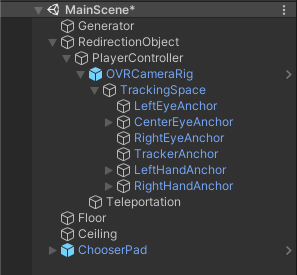
\includegraphics[width=0.5\textwidth]{images/hierarchy.png}
    \caption{Die Hierachie der Unity-Szene vor der Laufzeit}
\end{figure}

\section{Design der Szene}
%TODO: Bild von Raum
Im folgenden werde ich die Designentscheidungen, die die Optik der Szene bestimmen erläutern.

Die virtuelle Umgebung, die die Nutzer:in durchschreitet ist der eines Dungeons nachempfunden. Dies ist in Computerspielen ein häufig eingesetztes Setting, weltbekannte Spiele wie
\textquote{The Elder Scrolls V: Skyrim}, %TODO: sources?
die \textquote{Final Fantasy} Spielreihe,
die \textquote{The Legend of Zelda} Spielreihe,
und besonders sogenannte \textquote{Roguelike}-Spiele, wie
die \textquote{Diablo} Spielreihe,
\textquote{The Binding of Isaac},
oder \textquote{Darkest Dungeon}, beinhalte alle zumindest zum Teil Dungeonartige Level, die den Spieler herausfordern eine dunkle Umgebung zu erkunden und gegen fiese Gegner zu kämpfen.
Obgleich letzteres in den hier erzeugten Leveln nicht vorkommt, ist das  Ambiente bewusst ein wenig düster gehalten und erinnert optisch an einen Dungeon. Sehr hilfreich ist dafür die aus dem Unity-Asset-Store heruntergeladene Textur \cite{dungeon-material}, die die Wände schmückt und ihnen ein rustikales, dungeonartiges Gefühl verleihen.

Das Spiel \textquote{Rogue}, von 1980, nachdem auch das Genre \textquote{Roguelike} benannt wurde ist ein Meilenstein in der Prozeduralen Levelgeneration gewesen und hat bis heute großen Einfluss auf die Welt der Computerspiele. Auch dabei geht es darum einen Dungeon zu erkunden, auch wenn dieser verständlicherweise graphisch, noch nicht besonders aufbereitet gewesen ist.

Abgesehen davon bietet die Umgebung eines Dungeons viele Freiheiten, was den Realismus der Welt angeht. Es wird nicht hinterfragt wieso ein Gebäude so strukturiert sein sollte, dass man die ganze Zeit um die Ecke geht oder wieso die Türen sich öffnen und schließen, in dem sie magisch erscheinen oder sich auflösen.

Um die Erkundungsstimmung noch ein wenig zu verstärken und eine realistische Lichtquelle in die Welt einzubauen trägt die Nutzer:in eine Kopflampe, dies ist ein einfacher Spotlight mit leicht bläulichem Licht, dessen Parent die Kamera des Spieler:innenavatars ist.

%MCI mässige quellen wären hier gut

%section hände, avatar etc

\section{Implementierung der Rotationgains}

Die Umsetung der Rotaiongains erfolgt mithilfe des
%TODO: Von wem genau kommt space extender?
freundlicherweise zur Verfügung gestelltem Unity-Package \textquote{Space-Extender}. Dieses bietet das Prefab \textquote{RotationRedirector}, welches im Code instanziiert werden kann und dann nachdem es richtig positioniert ist, die Dimensionen des Trackingspaces und den virtuellen Avatar der Nutzer:in und die Kooridinaten, des Punktes, um den rotiert werden soll übergeben bekommen hat, dazu in der Lage ist einen Rotationgain auf die Nutzer:in anzuwenden. Der RotationRedirector wird nachdem das alles geschehen ist für jeden Raum, an die Instanz des RotationGainMechanism, die für eben jenen Raum zuständig ist übergeben, sodass er aktiviert werden kann sobald das Signal vom ensprechenden Collider kommt, dass die Nutzer:in sich über dem Rotationspunkt ($P$) befindet.

\section{Der Rotationgain Inzentivierungs Mechanismus}
\label{sec:rotgaininc}

Damit der Rotationgain seinen Effekt erzielen kann ist es wichtig, dass die Nutzer:in sich etwa auf den Punkt $P$ stellt und ihren Kopf um die Y-Achse dreht.
Damit sich dies intuitiver anfühlt und die Aufmerksamkeit nicht so konkret auf den Rotationgain gelenkt wird, habe ich mich dagegen entschieden den Nutzer:innen einfach den Punkt $P$ zu markieren und sie zu bitten dort ihren Kopf zu drehen, sondern habe mir einen Vorwand ausgedacht, wieso es zum einen Notwendig ist an der Stelle zu stehen und zum anderen, wieso sie ihren Kopf drehen müssen.

%TODO: NumPad Picture
Um diesen Effekt zu erzielen wird ein Nummern-Eingabefeld, an der Korridorinnenwand in Richtung des Raumes aus dem die Nutzer:in gerade kommt, genau vor die Position $P$ plaziert. In dieses Eingabefeld sollen dann mehrere zweistellige Nummern, die am anderen Ende des Korridors, auf einer digitalen Tafel angezeigt werden eingegeben werden, bis die Tür sich öffnet. Auf der Tafel wird nur eine zweistellige Nummer zur Zeit angezeigt.
Dies sorgt dann sowohl dafür dass die Nutzer:in sich automatisch auf den Punkt $P$ stellt, um möglichst gut die Nummern eingeben zu können, als auch dafür, dass die Nutzer:in ihren Kopf wiederholt um die Y-Achse dreht weil sie abwechselnd ablesen muss welche Zahlen auf der Tafel hinter ihr angezeigt werden und dann die Zahlen in das Eingabefeld schräg vor ihr eingeben muss. Dies sorgt für einen intuitiven Grund den Kopf zu drehen und somit dafür den Rotationgain zu nutzen. Wenn der Fortschritt des Rotation-Gains abgeschlossen ist und ein weiteres Mal die korrekte Nummer in das Eingabefeld eingegeben wurde, öffnet sich die Tür vor der Nutzer:in (also die \textquote{Seitentür}) sodass die Nutzer:in in den nächsten Raum gehen kann. Da nun der Trackingspace genau den nächsten Raum umgibt ist es wichtig, dass die Nutzer:in nicht versucht zurück in den vorherigen Raum zu gehen. Aus diesem Grund schließt sich hinter der Nutzer:in eine vorher noch nicht zu erkennenende Tür.

Im Programm-Code findet sich dieser ganze Vorgang in der Klasse \textquote{RotationGainMechanism}. Dieser wird für jeden Raum erstellt und auch dem Objekt des Raumes als Component hinzugefügt. Eine Instanz des RotationGainMechanisms ist also immer für den Raum zuständig auf dem er sich befindet. Mit der \textquote{Init}-Funktion wird das Objekt direkt nach der Erstellung initialisiert, hier meldet sich die Instanz dann auch in der zugehörigen Eingabefeld-Klasse (\textquote{NumPadScript}) als Observer an. Sobald sich die Nutzer:in dann in den um die Position $P$ herum platzierten Collider wird mit der Funktion \textquote{StartMechanism} die Prozedur gestartet. Zunächst wird eine neue zweistellige Zahl mithilfe des (von Unity bereitgestellten) Pseudozufallgenerators erstellt, dann wird diese Zahl auf der dem aktuellen Raum zugehörigen Tafel angezeigt. Sobald die Bestätigungstaste des Eingabefelds gedrückt wurde (\textquote{$\#$}), wird überprüft ob der Fortschritt des Rotation-Gains schon bei 100\% ist. Falls nicht, beginnt das ganze von vorne und es wird eine neue Zahl erstellt. Wenn der Rotation-Gain vollständig abgeschlossen ist (also eine 90\textdegree\ Drehung stattgefunden hat) wird dem \textquote{RoomAndProgressManager} mitgeteilt dass der aktuelle Raum abgeschlossen ist und die Tür öffnet sich.

In den Kontrollbedingungen wird kein Rotationgain angewandt. Dennoch müssen die Proband:innen auch hier Zahlen in das Eingabefeld eingeben. In diesen Szenarien wird die Türöffnung aus offensichtlichen Gründen nicht von der vervollständigung des Rotationgains abhängig gemacht, sondern wird eine Zufallszahl zwischen 4 und 8 bestimmt und mitgezählt, wie oft Zahlen bestätigt wurden. Wenn die Zufallszahl erreicht wird öffnet sich die Tür. Durch die Erfahrung beim Testen hat sich gezeigt dass es etwa zwischen 4 und 8 Eingaben bedarf, bevor der Rotationgain abgeschlossen ist.

\section{Messmechanismen und Datenspeicherung}
Um an späterer Stelle einschätzen zu können, wie gut die Proband:innen die Entfernung die sie sich fortbewegt haben geschätzt haben ist es notwendig eben dies auch zu messen. Zusätzlich dazu ist es auch notwendig diese Daten zu speichern. Im folgenden werde ich erläutern, wie dies implementiert ist.

Da es nicht darum geht die Luftlinie zwischen Start und Ende des Levels zu messen, da dann die Bewegungsweise der Proband:in keine Rolle mehr spielen würde, sondern ihre konkreten Fortbewegungsstrecke zu messen, ist diese Aufgabe nicht gänzlich trivial. Würde man einfach in jedem Frame die Kopfposition des virtuellen Avatars, der Proband:in speichern, die Distanz zum vorherigen Punkt berechnen und aufsummieren, wäre das Ergebnis sehr unexakt. %?
Da nun jede millimeterbewegung des Kopfes aufsummiert werden würde, würde eine einfache Kopfdrehung die fortbewegte Strecke schon um einen großen Teil erhöhen. Dies würde dazuführen, dass die Messung der fortbewegten Strecke nicht mehr intuitiv einzuschätzen wäre.
Um dem entgegenzuwirken habe ich die Auflösung dieser Messung deutlich veringert, indem nicht mehr jedes Frame, diesen Prozess durchläuft, sondern nur ein Frame etwa alle 2 sekunden. So werden deutlich grobere Bewegungen gemessen und die gemessenen Ergebnisse passen deutlich besser zu der intuitiven Einschätzung der Entfernung.
%TODO: zu unwissenschaftlich? nochmal best practices recherchieren

All dies ist im \textquote{RoomAndProgressManager} implementiert. Hier gibt es eine \textquote{StartTimeMeasure}-Methode, die zum Start der Bedingung vom \textquote{SceneLoader} aufgerufen wird und eine \textquote{AddDistance}-Methode, die in der von der \textquote{Update}-Methode alle 150 Frames einmal aufgerufen wird. Diese bestimmt dann euklidisch die Distanz zwischen der aktuellen Position der Nutzer:in und der zuletzt gemessenen und addiert diese auf eine Kummulationsvariable.

Sobald das Level der Versuchsbedingung abgeschlossen ist wird diese Kummulationsvariable an den \textquote{FirebaseHandler} weitergeleitet, der nun die Daten der aktuellen Versuchsbedingung an die private Datenbank sendet um die Daten für die spätere Auswertung zu speichern.

\chapter{Levelgenerierung}
\label{section:generate}
Dieses Kapitel beschreibt, wie genau die Generierung eines in diesem Projekt genutzen Levels funktioniert. Nacheinander werde ich die grundlegenden Ideen hinter der Levelgenerierung erörtern und dabei jeweils genauer auf ihre Implementierung eingehen um dann den Algorithmus, der die unterschiedlichen Codeblöcke nutzt um die Levelstruktur zu generieren, zu beschreiben und vorzustellen.
Zuerst wird besprochen, wie die Räume angeordnet werden müssen damit sie durch den Rotation-Gain verbunden werden können. Dann wird erklärt und vorgestellt wie die Korridore, die in den Räumen generiert werden um der Nutzer:in einen klaren Weg voran zu präsentieren und den Übergang zwischen den Räumen intuitiver zu gestalten, erstellt werden. Als nächstes beschreibe ich die Vorgänge die für die Generierung der Wände der Räume verantwortlich sind und erkläre wie die entsprechenden Berechnungen stattfinden.
Um hinterher dann den Generierungs-Algorithmus und den zugehörigen Quelltext vorzustellen wird dann noch Beschrieben an welchen Stellschrauben manipuliert werden kann um heterogene Ergebnisse zu bekommen, erst hier können (Pseudo-)Zufallsfaktoren eine Rolle spielen.
Den krönenden Abschluss dieses Kapitel bekommt dann der Abschnitt,
der die Zusammensetzung des Algorithmusses zunächst erklärt und den entsprechenden Quelltext dann auch noch ausführlich vorstellt.

\section{Raumplatzierung}

Um zu verstehen wie die Berechnung der Ecken eines Raumes funktioniert ist es zunächst essentiell, die Grundidee hinter der Raumanordnung zu verstehen.

\begin{figure}[H]
    \ctikzfig{2rooms_a}
    \caption{Veranschaulichung der Raumstellung zueinander, sodass $P$ den Drehpunkt kennzeichnet }\label{figure:two_rooms} %TODO: formulierung
    %TODO: P is a point
\end{figure}

%paragraph Erklärung
\subsection{Grundidee}
\label{subsec:roomplaceidea}
%Um die durchgehende Weiterführung des Levels zu ermöglichen werden zwei Räume immer genau so angeordnet, dass ein Rotation-Gain, der genau bis zu einer Verdrehung der beiden Realitäten von 90\textdegree\ angewandt wird, während die Nutzer:in an einem bestimmten Punkt in der Ecke des Raumes steht,
Wenn ein Rotation-Gain angewandt wird verdrehen sich virtuelle und reale Realität um den Drehpunkt, der durch die Position der Nutzer:in bestimmt wird. Wenn diese Position $P$ sich in einer Ecke des (rechteckigen) Raumes befindet, zudem genau gleich weit von beiden Wänden, die diese Ecke bilden, entfernt ist und auf die Nutzer:in dann ein Rotation-Gain angewandt wird,
bis genau 90\textdegree\ Verdrehung erreicht sind, dann steht der aktuelle Bereich in der virtuellen Realität der vom realen Trackingspace begrenzt ist $A$, dem vorherigen Bereich, der durch den Trackingspace begrenzt war $B$ genau orthogonal gegenüber.
Die beiden Areale $A$ und $B$ überlappen sich in einem gewissen Bereich, in dem die Nutzer:in nach Beendigung des Rotation-Gains dann gerade steht, aber ein Großteil von $B$ ist Teil der virtuellen Realität der zuvor nicht zugänglich war. Auf diese Weise ist also für die Nutzer:in ein neuer Bereich der Virtuellen Welt begehbar geworden.
Da ja aber ein Rotation-Gain angewandt wurde hat die Nutzer:in nicht bewusst wahrgenommen, dass die Welten sich verdreht haben. Wenn sie nun also geradeaus geht entsteht dann der Eindruck, dass nun ein weiterer Teil der Welt zugänglich geworden ist.
Ziel des Algorithmus ist es eine Reihe von aufeinander folgenden Räumen zu generieren, sodass die Nutzer:in sich durch ein Dungeon-artiges Level bewegen kann um vom ersten zum letzten Raum zu gelangen.
Die Grundidee hinter der Raumgenerierung ist es also, dass genau die beiden Areale $A$ und $B$ von Wänden umgeben werden. %TODO: formulierung
In \autoref{figure:two_rooms} wird ersichtlich, wie die beiden Räume zueinander Stehen müssen um diesen Effekt zu ermöglichen.

Um dann also von Raum $A$ zu Raum $B$ zu kommen muss die Nutzer:in sich an der Position $P$ oft genug drehen und ein Rotation-Gain bis zu 90\textdegree\ angewandt werden.
Danach kann sie mit der Illusion geradeaus zu gehen einen neuen Raum erkunden während sie sich eigentlich nur weiter innerhalb des realen Trackingspaces bewegt. Der reale Trackingspace umschließt also immer genau den Raum in dem sich die Nutzer:in gerade befindet.

\subsection{Berechnung der Ecken}
\label{subsection:calccorners}

\begin{figure}[H]
    \centering
    \begin{tikzpicture}
	\begin{pgfonlayer}{nodelayer}
		\node [style=none] (37) at (-7, 7) {};
		\node [style=none] (38) at (1, 7) {};
		\node [style=none] (39) at (-7, -3) {};
		\node [style=none] (40) at (1, -3) {};
		\node [style=none] (41) at (-1, 7) {};
		\node [style=none] (42) at (9, 7) {};
		\node [style=none] (43) at (-1, -1) {};
		\node [style=none] (44) at (9, -1) {};
		\node [style=none] (0) at (0, 7) {};
		\node [style=none] (18) at (9, -1) {};
		\node [style=none] (19) at (-1, -1) {};
		\node [style=none] (20) at (9, 7) {};
		\node [style=none] (21) at (-1, 7) {};
		\node [style=none] (45) at (-1, 6) {};
		\node [style=none] (47) at (-1, 6) {};
		\node [style=none] (50) at (0.25, 6.5) {$dP$};
		\node [style=none] (51) at (-0.5, 5.75) {$dP$};
		\node [style=none] (52) at (0, 6) {};
		\node [style=none] (53) at (0.25, 5.75) {$P$};
		\node [style=none] (55) at (-1.25, 6) {$cP$};
		\node [style=none] (57) at (9, 7.25) {$C_b$};
		\node [style=none] (58) at (-1, 7.25) {$C_a$};
		\node [style=none] (59) at (-1, -1.25) {$C_d$};
		\node [style=none] (60) at (9, -1.25) {$C_c$};
	\end{pgfonlayer}
	\begin{pgfonlayer}{edgelayer}
		\draw [style=new edge style 0] (40.center)
			 to (39.center)
			 to (37.center)
			 to (38.center)
			 to cycle;
		\draw [style=new edge style 1] (43.center)
			 to (41.center)
			 to (42.center)
			 to (44.center)
			 to cycle;
		\draw [style=arrow] (21.center) to (47.center);
		\draw [style=arrow] (19.center) to (47.center);
		\draw [style=arrow] (18.center) to (19.center);
		\draw [style=arrow] (20.center) to (21.center);
		\draw [style=dashes] (52.center) to (0.center);
		\draw [style=arrow] (45.center) to (52.center);
        \draw [decorate,decoration={brace,mirror,amplitude=10pt}](-1,-1.5) -- (9,-1.5) node [midway,yshift=-0.25in] {$length$};
        \draw [decorate,decoration={brace,amplitude=10pt}](-1.5,-1) -- (-1.5,7) node [midway,xshift=-0.40in] {$width$};
	\end{pgfonlayer}
\end{tikzpicture}

    \caption{Zur Eckenberechnung genutzte Vektoren. Mit $C_{0-3}$ werden die Ecken bezeichnet, mit $S_{0-3}$ die Seiten des Raumes (Nicht die zur Eckenberechnung genutzen Vektoren). }
    \label{figure:calculateCornersFig}
\end{figure}

Um dies umzusetzen müssen zunächst die Koordinaten der Ecken innerhalb der virtuellen Umgebung bestimmt werden. Für den ersten Raum ist es nicht schwierig, die virtuellen Koordinaten der Ecken der Trackingspace-Boundaries werden vom Oculus Integration SDK geliefert.
In der \textquote{GeneratorOculusInterface} Klasse werden diese zu Beginn der Levelgenerierung abgefragt und der \textquote{GenerateLevel}-Klasse zur Verfügung gestellt. Um allerdings die Raumecken der folgenden Räume zu bestimmen müssen die Position $P$ sowie der Abstand von $P$ zu den Wänden des jeweiligen Vorraums definiert sein( $dP$ ). Die Berechnung dieser Punkte findet sich in \autoref{sec:corridor}. Für die weiteren Räume berechnen sich die Eckvektoren, dann folgendermaßen. Auch zu sehen ist diese Berechnung in dem in der \autoref{figure:calculateNewCornersScript} gezeigen Quelltext.

% $$ cP = P + (-1) * sDD * dP $$

% $$ C_a = cP + (-1) * btF * dP $$
% $$ C_b = C_a + sDD * length $$
% $$ C_c = C_d + sDD * length $$
% $$ C_d = cP + btF * (width - dP) $$

    \begin{align}
        \begin{split}\label{eq:1}
            cP ={}& P + (-1) * sDD * dP
        \end{split}\\ \\
        \begin{split}\label{eq:2}
            C_0 ={}& cP + (-1) * btF * dP
        \end{split}\\
        \begin{split}\label{eq:3}
            C_1 ={}& C_a + sDD * length
        \end{split}\\
        \begin{split}\label{eq:4}
            C_2 ={}& C_d + sDD * length
        \end{split}\\
            C_3 ={}& cP + btF * (width - dP)\label{eq:5}
        \end{align}

    % \begin{align}
    %     \begin{split}\label{eq:1}
    %         a ={}& b + c + d\\
    %              & + e + f + g
    %     \end{split}\\
    %     \begin{split}\label{eq:2}
    %         k ={}& l + m + n + m + n + m + n\\
    %              & + o + p + q
    %     \end{split}\\
    %         r ={}& s + t (u + v + w)\label{eq:3}
    %     \end{align}

Wie die hier genutzen Variablen $cP$, $sDD$, $btF$, $width$ und $length$ definiert sind wird aus \autoref{figure:calculateCornersFig} ersichtlich. $cP$ steht dabei für den Punkt hinter $P$, der genau eine $dP$ länge in Richtung des alten Raumes liegt. $sDD$ (sideDoorDirection) ist ein normalisierter Richtungsvektor, der die Richtung des Korridors des letzen Raumes erweitert. $btF$ (backToFront) ist auch ein normalisierter Richtungsvektor, der orthogonal zu $sDD$ steht. Er zeigt von der hinteren Wand des Korridors des vorherigen Raumes zur vorderen Wand. $width$ beschreibt die Breite der Räume, während $length$ die Länge beschreibt. Diese beiden Variablen hängen von den Maßen des ersten Raumes ab, bei dem die Eckkoordinaten ja den Trackingspace der Nutzer:in abbilden. Wichtig ist noch zu erwähnen, dass die in der eben erwähnten Abbildung gezeigte Folge von Ecken und Seiten, nicht genau spiegelverkehrt ist wenn der Raum in die andere Richtung generiert würde (siehe \autoref{sec:random}), sondern die Reihenfolge der Ecken genau andersherum läuft. Das ganze ist also nicht nur vertikal, sondern auch horizontal gespiegelt zu der Darstellung.

\begin{figure}[H]
    \centering
    \sourcecode{calculateNewCorners.cs}
    \caption{Funktion zur Berechnung der virtuellen Eckkoordinaten des nächsten Raumes}
    \label{figure:calculateNewCornersScript}
\end{figure}


\section{Korridore}
\label{sec:corridor}
%paragraph Erklärung
%TODO: Bild eines Korridors
Damit die Nutzer:in versteht wie sie in den nächsten Raum kommt sind die Räume so designed, dass es einen offensichtlichen Weg voran gibt. Um dies zu erreichen wird eine Kante des Grundecks des Raumes ausgewählt, an der ein Korridor erstellt wird (diese wird Pseudozufällig ausgewählt, siehe \autoref{sec:random}). Er kann sowohl an einer kürzeren Kante als auch an einer längeren Kante des Grundecks des Raumes erstellt werden, nur nicht an der Seite an der das Ende des Korridors des letzten Raums herausragt.
Der Korridor hat zwei Türen; Eine \textquote{Haupttür}, durch die die Nutzer:in in den Korridor hineinkommt und eine \textquote{Seitentür}, die anfangs noch verschlossen ist und in den nächsten Raum führt.

In diesem Korridor werden dann Elemente platziert die gemeinsam für einen Mechanismus sorgen, der die Nutzer:in inzentiviert sich genug zu drehen, dass die wirkliche und die virtuelle Realität sich dank des Rotation-Gains genug umeinander drehen, dass der nächste Raum nun mit dem realen Tracking-Space übereinstimmt. Dieser Mechanismus wird in
\autoref{sec:rotgaininc}
genauer beschrieben.

\subsection{Korridor-Meshgenerierung}
\label{subsec:corridormesh}
Um einen solchen Korridor zu generieren müssen zunächst die Koordinaten der genutzten Vertices %TODO: genauer erklären?
bestimmt werden. Zudem müssen dann entsprechende Faces gespannt und für jeden Vertex dann auch die UV-Koordinaten errechnet werden. All dies geschieht in der \textquote{RoomGenerator}-Klasse.

Ein Korridor besteht aus einem Boden, einer Frontalwand, zwei Seitenwänden und einer Rückwand.
Bevor die Meshgenerierung stattfinden kann muss zunächst die Variable $D$ bestimmt werden. Dabei handelt es sich um einen Wert zwischen $0$ und $1$, der für jeden Raum (Pseudo-)zufällig generiert wird (siehe \autoref{sec:random}). Mit diesem Wert werden die Türpositionen bestimmt, je geringer er ist desto weiter links liegt die Haupttür in der Frontalwand. Ist der Wert geringer als 0.5 befindet sich die Seitentür in der rechten Seitenwand, sonst in der linken, sodass diese immer auf der gegenüberliegende Seite der Haupttür liegt.

Es gibt zwei Möglichkeiten der Struktur einer Wand, abhängig davon ob in ihr eine Tür liegt oder nicht. Der simplere Fall trifft zu wenn in der Wand keine Tür liegt, dann besteht die Wand aus 8 Vertices.
Die Wandstruktur der Alternative wird in \autoref{figure:doorCalcFig}
veranschauligt. Dabei ist allerdings zu beachten, dass nur die Frontalansicht auf eine solche Wand gezeigt ist, die Innenseite derselben Wand hat allerdings die selbe Struktur. Zudem sind die Vertices der Tür jeweils mit ihren inneren Gegenspielern durch Faces verbunden, sodass man beim durchschreiten der Tür nicht ins innere der Wand blicken kann.

\paragraph*{Vertices}

Das Generieren eines solchen Korridors läuft dann also wie folgt ab. Gegeben sind die die Eckkoordinaten des Raumes in den der Korridor platziert werden soll ($C_{a-d}$), die Seite des Raumes, an der der Korridor liegen soll $S$ ($_{a-d}$), die Türposition $D$, die Tiefe des Korridors $d$, durch die sich der in \autoref{subsection:calccorners} besprochene Abstand des Punktes $P$ zu den Wänden der Ecke des Punktes ergibt: $d = 2 * dP$, die Höhe $h$ und Dicke der Wände $w$ sowie die Höhe ($dh$) und Breite ($dw$) der Tür .

Als erstes werden die unteren, äußeren Punkte berechnet. ($F_{1-4}$)
Dabei wird mit den beiden hinteren, äußeren Punkte des Korridors begonnen. Da die Ecken eines Raumes immer im Uhrzeigersinn gespeichert werden lassen sich die Ecke des Raumes, die $S$ entspricht, und die im Uhrzeigersinn darauf folgende auswählen. %TODO: formulierung

$$ F_1 = C_S $$
$$ F_2 = C_{(S+1) \% 4} $$ %modulo???

Damit wird der Richtungsvektur $rTL$ bestimmt indem die rechte Ecke von der linken Ecke subtrahiert wird und das Ergebnis dann normalisiert wird.

$$ rTL = F_2 - F_1 $$ %TODO: normalisieren?

Um die beiden vorderen äußeren Ecken zu bestimmen muss nun ein richtungs Vektor $tF$ berechnet werden der von der Seite $S$ in Richtung der gegenüberliegenden Seite des Raumes zeigt. Hierfür wird das Kreuzprodukt von $rTL$ und dem Vektor
%vektor nach oben einfügen
berechnet und das Ergebnis normalisiert.

$$ tF = rTL x $$ %TODO: oben vektor, kreuzprodukt, normalisieren

Um nun die vorderen Punkte zu bestimmen wird einfach der neue Richtungsvektor mit $2 * dP$ multipliziert und auf die hinteren Punkte addiert.

$$F_3 = F_1 + tF * dP $$
$$F_4 = F_2 + tF * dP $$

Nach demselben Prinzip lassen sich nun die äußeren oberen Ecken des Korridors bestimmen, hierfür werden die unteren Ecken mit dem Vektor $T$ addiert, der sich wie folgt berechnet:

$$T = up * h $$ %TODO: up

Um die inneren Punkte zu berechnen werden die äußeren Ecken nach dem selben Prinzip, jeweils mit den beiden Richtungsvektoren, die beide mit $w$ multipliziert werden addiert.


\begin{figure}[H]
    \centering
    \begin{tikzpicture}
	\begin{pgfonlayer}{nodelayer}
		\node [style=none] (0) at (-5, 4) {};
		\node [style=none] (1) at (5, 4) {};
		\node [style=none] (2) at (5, 0) {};
		\node [style=none] (3) at (-5, 0) {};
		\node [style=none] (4) at (3, 0) {};
		\node [style=none] (5) at (3, 4) {};
		\node [style=none] (6) at (2.25, 0) {};
		\node [style=none] (7) at (-4.25, 0) {};
		\node [style=none] (8) at (-2.75, 0) {};
		\node [style=none] (9) at (-1.25, 0) {};
		\node [style=none] (10) at (-2.75, 3) {};
		\node [style=none] (11) at (-1.25, 3) {};
		\node [style=none] (12) at (-2.75, 4) {};
		\node [style=none] (13) at (-1.25, 4) {};
		\node [style=Point] (14) at (-2, 0) {};
		\node [style=Point] (15) at (4, 0) {};
		\node [style=Point] (16) at (3, 0) {};
		\node [style=Point] (17) at (2.25, 0) {};
		\node [style=Point] (18) at (-4.25, 0) {};
		\node [style=none] (20) at (3, -0.5) {$xP$};
		\node [style=none] (21) at (-2, -0.5) {$mD$};
		\node [style=none] (22) at (4, -0.5) {$P$};
	\end{pgfonlayer}
	\begin{pgfonlayer}{edgelayer}
		\draw [style=dashes] (3.center) to (12.center);
		\draw [style=dashes] (9.center) to (1.center);
		\draw [style=dashes] (10.center) to (13.center);
		\draw [style=dashes] (0.center) to (12.center);
		\draw [style=dashes] (0.center) to (3.center);
		\draw [style=dashes] (12.center) to (8.center);
		\draw [style=dashes] (3.center) to (8.center);
		\draw [style=dashes] (12.center) to (13.center);
		\draw [style=dashes] (13.center) to (11.center);
		\draw [style=dashes] (13.center) to (1.center);
		\draw [style=dashes] (11.center) to (9.center);
		\draw [style=dashes] (10.center) to (11.center);
		\draw [style=dashes] (9.center) to (2.center);
		\draw [style=dashes] (1.center) to (2.center);

        \draw [decorate,decoration={brace,amplitude=7.5pt}](4,0.5) -- (5,0.5) node [midway,yshift=0.5cm] {$dP$};

        \draw [decorate,decoration={brace,amplitude=7.5pt}](3,0.5) -- (4,0.5) node [midway,yshift=0.5cm] {$dP$};

        \draw [decorate,decoration={brace,amplitude=7.5pt}](2.25,0.5) -- (3,0.5) node [midway,yshift=0.5cm] {$dw / 2$};

        \draw [decorate,decoration={brace,amplitude=7.5pt}](-5,0.5) -- (-4.25,0.5) node [midway,yshift=0.5cm] {$dw / 2$};

        \draw [decorate,decoration={brace,amplitude=7.5pt}](-2.75,0.5) -- (-1.25, 0.5) node [midway,yshift=0.5cm] {$dw$};

        % \draw [decorate,decoration={brace,mirror,amplitude=10pt}](-4.25,-1) -- (3, -1) node [midway,yshift=-0.75cm] {$mDX$};

        % türhöhe brace
        \draw [decorate,decoration={brace,amplitude=10pt}](-3,0) -- (-3,3) node [midway,xshift=-0.75cm] {$dh$};

        % door vektors
        \draw [style=arrow](-2.75,0) -- (-2, 0);
        \draw [style=arrow](-2.75,3) -- (-2, 0);
        \draw [style=arrow](-1.25,0) -- (-2, 0);
        \draw [style=arrow](-1.25,3) -- (-2, 0);

        \draw [style=arrow](-4.25,-1) -- (3, -1) node [midway,yshift=-0.5cm] {$mDX$};


	\end{pgfonlayer}
\end{tikzpicture}

    \caption{} %TODO:caption
    \label{figure:doorCalcFig}
\end{figure}

Für die Tür-Vertices wird zunächst der untere Mittelpunkt der Tür ($mD$) berechnet.
In der folgenden Erklärung wird davon ausgegangen, dass $D <= 0.5$ ist und somit die Haupttür links, und die Seitentür rechts erzeugt wird, andernfalls  wären natürlich $lTR$ und $rTL$ vertauscht.
Hierfür ist es zunächst wichtig die entsprechende Achse ($mDX$)zu berechnen, auf der die Tür dann erzeugt wird (siehe \autoref{figure:doorCalcFig})

Dafür wird erstmal der Punkt, an der Frontalseite des Korridors, diagonal hinter $P$ berechnet ($xP$). Von da aus spannt sich die Achse dann bis zur anderen Seite des Korridors. Da $mD$ ja den Mittelpunkt der Haupttür darstellen soll, muss an beiden Seiten der Achse $dw / 2$ als padding eingesetzt werden, damit die Tür nicht weiter oder rechts übersteht, falls $D$ einen extremwert annimmt. $mD$ berechnet sich dann folgendermaßen:

$$ mD = xP + D * mDX $$

Die Berechnung von $xP$, und $mDX$ wird aus dem in \autoref{figure:calcMainDoorCode}
dargestellten quelltext ersichtlich. %kommentare, variablen übersetzen etc.

Die Berechnung der Vertices, in der Haupttür ist nun trivial und erfolgt mit der bekannten Methode und wird auch in \autoref{figure:doorCalcFig} ersichtlich. Türhöhe ($dh$), Türbreite ($dw$) und Wandbreite ($w$) werden mit den entsprechenden Richtungsvektoren multipliziert und auf $mD$ addiert.
%TODO: side door

\begin{figure}[H]
    \centering
    \sourcecode{calcMainDoor.cs}
    \caption{} %TODO:caption
    \label{figure:calcMainDoorCode}
\end{figure}

\paragraph*{Faces}
Der nächste Schritt, der für die Meshgenerierung erforderlich ist, ist das Spannen der verschiedenen Faces (Triangles). Die meisten für den Korridor erforderlichen Flächen bestehen nur aus zwei aneinanderliegenden Triangles, die somit gemeinsam die viereckige Fläche bilden. Die Ausnahmen, sind die Frontalfläche und die Seitenfläche in die die Seitentür generiert wurde (jeweils mit der zugehörigen Innenseite). Die Struktur dieser Flächen wird auch in \autoref{figure:doorCalcFig} ersichtlich. Auch hier werden die benötigten Vertices jeweils durch multiplizieren mit den entsprechenden Richtungsvektoren und der anschließenden Addierung auf bestehende Vertices errechnet.

Um die späteren UV Berechnungen nicht zu verunreinugen wird jeder Vertex dem Buffer pro Face einmal hinzugefügt. Die Faces werden dann gespannt indem die jeweiligen Indizes der Vertices im Buffer aufgelistet werden. Dies beides wird dann dem neu erzeugten $MeshFilter$ Objekt übergeben.

\paragraph*{UV}
Die Berechnung der UV-Koordinaten erfolgt für jeden einzeln und wird nach Triangles geordnet der Reihe nach durchgeführt. Der Quelltext dazu findet sich in der GenerateUV Methode, die in \autoref{figure:uvcode} Abgebildet ist.
Die Berechnung besteht daraus die Normale des Triangles zu berechnen, diese mit den Richtungsvektoren abzugleichen und die Vektoren der Vertices dann entsprechend zu Rotieren.

\begin{figure}[H] %TODO: more pages
    \centering
    \sourcecode{uvCode.cs}
    \caption{} %TODO:caption
    \label{figure:uvcode}
\end{figure}



\section{Wandgenerierung}
\label{sec:genwalls}
%paragraph Erklärung
Natürlich reichen die Meshs der Korridore noch nicht aus um das Gefühl eines Raumes zu vermitteln, zumal diese ja auch nur an einer Seite des Raumes statuiert sind.
Wie in \autoref{subsec:roomplaceidea} besprochen sollen die Räume von Wänden umgeben sein.

\begin{figure}[H]
    \centering

    \scalebox{0.4}{\begin{tikzpicture}
	\begin{pgfonlayer}{nodelayer}
		\node [style=none] (0) at (10, 16) {};
		\node [style=none] (1) at (10, 0) {};
		\node [style=none] (2) at (-8, -3) {};
		\node [style=none] (3) at (0, -3) {};
		\node [style=none] (4) at (-8, -13) {};
		\node [style=none] (5) at (0, -13) {};
		\node [style=none] (6) at (-2, -3) {};
		\node [style=none] (8) at (-2, -11) {};
		\node [style=none] (10) at (0, -3) {};
		\node [style=none] (13) at (0, -5) {};
		\node [style=none] (14) at (-8, -5) {};
		\node [style=none] (15) at (-5, -5) {};
		\node [style=none] (16) at (-7, -5) {};
		\node [style=none] (17) at (-5, -4.75) {};
		\node [style=none] (18) at (-5, -5.25) {};
		\node [style=none] (19) at (-7, -4.75) {};
		\node [style=none] (20) at (-7, -5.25) {};
		\node [style=none] (21) at (0, -3.25) {};
		\node [style=none] (22) at (-0.25, -3.25) {};
		\node [style=none] (23) at (0.25, -3.25) {};
		\node [style=none] (24) at (0.25, -4.75) {};
		\node [style=none] (25) at (0, -4.75) {};
		\node [style=none] (26) at (-0.25, -4.75) {};
		\node [style=none] (28) at (-2, -11) {};
		\node [style=none] (32) at (-2, -9) {};
		\node [style=none] (33) at (3, -9) {};
		\node [style=none] (34) at (1, -9) {};
		\node [style=none] (35) at (3, -9.25) {};
		\node [style=none] (36) at (3, -8.75) {};
		\node [style=none] (37) at (1, -9.25) {};
		\node [style=none] (38) at (1, -8.75) {};
		\node [style=none] (46) at (-8, -3) {};
		\node [style=none] (47) at (0, -11) {};
		\node [style=none] (48) at (0, -9) {};
		\node [style=none] (49) at (-2, -5) {};
		\node [style=none] (50) at (6, -1) {};
		\node [style=none] (52) at (6, -11) {};
		\node [style=none] (58) at (6, -3) {};
		\node [style=none] (74) at (6, -1) {};
		\node [style=none] (79) at (10, 0) {};
		\node [style=none] (80) at (10, -16) {};
		\node [style=none] (81) at (10, 16) {};
		\node [style=none] (82) at (10, -1) {};
		\node [style=none] (83) at (10, -11) {};
		\node [style=none] (84) at (6, -1) {};
		\node [style=none] (85) at (10, -1) {};
		\node [style=none] (87) at (10, -11) {};
		\node [style=none] (89) at (6, -9) {};
		\node [style=none] (7) at (8, -3) {};
		\node [style=none] (90) at (-11, 16) {};
		\node [style=none] (93) at (-11, 0) {};
		\node [style=none] (9) at (8, -11) {};
		\node [style=none] (27) at (8, -11) {};
		\node [style=none] (31) at (8, -9) {};
		\node [style=none] (39) at (8, -10.75) {};
		\node [style=none] (40) at (7.75, -10.75) {};
		\node [style=none] (41) at (8.25, -10.75) {};
		\node [style=none] (42) at (8.25, -9.25) {};
		\node [style=none] (44) at (7.75, -9.25) {};
		\node [style=none] (86) at (8, -11) {};
		\node [style=none] (95) at (0, 13) {};
		\node [style=none] (96) at (-8, 3) {};
		\node [style=none] (97) at (0, 3) {};
		\node [style=none] (98) at (-2, 13) {};
		\node [style=none] (100) at (0, 13) {};
		\node [style=none] (101) at (0, 11) {};
		\node [style=none] (102) at (-8, 11) {};
		\node [style=none] (103) at (-5, 11) {};
		\node [style=none] (104) at (-7, 11) {};
		\node [style=none] (105) at (-5, 11.25) {};
		\node [style=none] (106) at (-5, 10.75) {};
		\node [style=none] (107) at (-7, 11.25) {};
		\node [style=none] (108) at (-7, 10.75) {};
		\node [style=none] (109) at (0, 12.75) {};
		\node [style=none] (110) at (-0.25, 12.75) {};
		\node [style=none] (111) at (0.25, 12.75) {};
		\node [style=none] (112) at (0.25, 11.25) {};
		\node [style=none] (113) at (0, 11.25) {};
		\node [style=none] (114) at (-0.25, 11.25) {};
		\node [style=none] (115) at (-2, 4.75) {};
		\node [style=none] (116) at (-2, 7) {};
		\node [style=none] (117) at (3, 7) {};
		\node [style=none] (118) at (1, 7) {};
		\node [style=none] (119) at (3, 6.75) {};
		\node [style=none] (120) at (3, 7.25) {};
		\node [style=none] (121) at (1, 6.75) {};
		\node [style=none] (122) at (1, 7.25) {};
		\node [style=none] (123) at (-0.5, 12) {$P$};
		\node [style=none] (124) at (-8, 13) {};
		\node [style=none] (125) at (0, 4.75) {};
		\node [style=none] (126) at (0, 7) {};
		\node [style=none] (127) at (-2, 11) {};
		\node [style=none] (130) at (6, 13) {};
		\node [style=none] (135) at (10, 15) {};
		\node [style=none] (136) at (8, 4.75) {};
		\node [style=none] (137) at (6, 7) {};
		\node [style=none] (139) at (8, 5) {};
		\node [style=none] (141) at (8, 7) {};
		\node [style=none] (142) at (8, 5) {};
		\node [style=none] (143) at (7.75, 5) {};
		\node [style=none] (144) at (8.25, 5) {};
		\node [style=none] (145) at (8.25, 6.75) {};
		\node [style=none] (146) at (8, 6.75) {};
		\node [style=none] (147) at (7.75, 6.75) {};
		\node [style=none] (147) at (7.75, 6.75) {};
		\node [style=none] (148) at (8, 5) {};
		\node [style=none] (149) at (8, 13) {};
		\node [style=none] (129) at (6, 4.75) {};
		\node [style=none] (131) at (6, 15) {};
		\node [style=none] (132) at (10, 15) {};
		\node [style=none] (133) at (10, 4.75) {};
		\node [style=none] (140) at (8, 4.75) {};
		\node [style=none] (150) at (0, 11) {};
		\node [style=Point] (152) at (-1, 12) {};
		\node [style=none] (153) at (-0.5, -4) {$P$};
		\node [style=Point] (154) at (-1, -4) {};
		\node [style=none] (155) at (10, 0) {};
		\node [style=none] (156) at (8, -9.25) {};
		\node [style=none] (157) at (10, 0) {};
		\node [style=none] (158) at (-11, -16) {};
	\end{pgfonlayer}
	\begin{pgfonlayer}{edgelayer}
		\draw [style=new edge style 0] (5.center)
			 to (4.center)
			 to (2.center)
			 to (3.center)
			 to cycle;
		\draw [style=new edge style 1] (8.center)
			 to (6.center)
			 to (7.center)
			 to (9.center)
			 to cycle;
		\draw [in=360, out=180] (10.center) to (46.center);
		\draw (17.center) to (18.center);
		\draw (19.center) to (20.center);
		\draw (13.center) to (15.center);
		\draw (16.center) to (14.center);
		\draw (23.center) to (22.center);
		\draw (24.center) to (26.center);
		\draw (10.center) to (21.center);
		\draw (25.center) to (13.center);
		\draw (35.center) to (36.center);
		\draw (37.center) to (38.center);
		\draw (41.center) to (40.center);
		\draw (27.center) to (39.center);
		\draw (46.center) to (14.center);
		\draw [style=wall] (5.center) to (47.center);
		\draw [style=wall] (5.center) to (4.center);
		\draw [style=wall] (14.center) to (4.center);
		\draw [style=wall] (13.center) to (48.center);
		\draw [style=dashed wall] (49.center) to (32.center);
		\draw [style=new edge style 0] (52.center) to (50.center);
		\draw [style=new edge style 0] (52.center)
			 to (27.center)
			 to (83.center)
			 to [in=270, out=90] (82.center)
			 to (74.center)
			 to cycle;
		\draw [style=wall] (48.center) to (47.center);
		\draw [style=new edge style 0] (58.center) to (74.center);
		\draw [style=new edge style 0] (74.center) to (58.center);
		\draw [style=new edge style 0] (74.center) to (58.center);
		\draw [style=new edge style 0] (84.center) to (85.center);
		\draw [style=dashed wall] (84.center) to (85.center);
		\draw [style=dashed wall, in=90, out=-90] (84.center) to (58.center);
		\draw [style=dashed wall] (86.center) to (87.center);
		\draw [style=dashed wall] (7.center) to (31.center);
		\draw [style=dashed wall] (10.center) to (7.center);
		\draw (90.center) to (81.center);
		\draw (1.center) to (93.center);
		\draw (93.center) to (90.center);
		\draw (86.center) to (39.center);
		\draw (41.center) to (40.center);
		\draw [style=new edge style 0] (97.center) to (96.center);
		\draw [style=new edge style 0] (95.center) to (97.center);
		\draw [style=new edge style 0] (150.center)
			 to (100.center)
			 to [in=360, out=180] (124.center)
			 to (102.center)
			 to (96.center)
			 to (97.center);
		\draw (105.center) to (106.center);
		\draw (107.center) to (108.center);
		\draw (104.center) to (102.center);
		\draw (111.center) to (110.center);
		\draw (112.center) to (114.center);
		\draw (100.center) to (109.center);
		\draw (113.center) to (101.center);
		\draw (119.center) to (120.center);
		\draw (121.center) to (122.center);
		\draw (144.center) to (143.center);
		\draw (145.center) to (147.center);
		\draw (140.center) to (142.center);
		\draw (146.center) to (141.center);
		\draw (116.center) to (115.center);
		\draw [style=wall] (97.center) to (125.center);
		\draw [style=new edge style 0] (130.center) to (131.center);
		\draw [style=new edge style 0] (131.center) to (130.center);
		\draw [style=new edge style 0] (131.center) to (130.center);
		\draw (141.center) to (146.center);
		\draw (145.center) to (147.center);
		\draw (148.center) to (142.center);
		\draw (144.center) to (143.center);
		\draw [style=new edge style 1] (136.center)
			 to (149.center)
			 to [in=360, out=180] (98.center)
			 to (115.center)
			 to [in=180, out=0] cycle;
		\draw [style=new edge style 0] (129.center)
			 to (140.center)
			 to (133.center)
			 to [in=270, out=90] (132.center)
			 to (131.center)
			 to cycle;
		\draw [style=new edge style 1] (150.center) to (100.center);
		\draw [style=new edge style 1] (150.center) to (100.center);
		\draw [style=wall] (96.center) to (102.center);
		\draw [style=wall] (96.center) to (97.center);
		\draw (102.center) to (124.center);
		\draw (124.center) to (98.center);
		\draw (98.center) to (100.center);
		\draw [style=wall] (116.center) to (127.center);
		\draw [style=wall] (100.center) to (130.center);
		\draw [style=wall] (131.center) to (132.center);
		\draw [style=wall] (130.center) to (131.center);
		\draw (147.center) to (146.center);
		\draw (145.center) to (147.center);
		\draw (144.center) to (143.center);
		\draw (142.center) to (140.center);
		\draw (141.center) to (146.center);
		\draw [style=wall] (137.center) to (130.center);
		\draw (150.center) to (113.center);
		\draw (112.center) to (114.center);
		\draw (100.center) to (109.center);
		\draw (111.center) to (110.center);
		\draw [style=wall] (140.center) to (133.center);
		\draw [style=dashed wall] (89.center) to (58.center);
		\draw (121.center) to (122.center);
		\draw (119.center) to (120.center);
		\draw [style=wall] (130.center) to (100.center);
		\draw (1.center) to (0.center);
		\draw (33.center) to (31.center);
		\draw (34.center) to (32.center);
		\draw (28.center) to (52.center);
		\draw (52.center) to (86.center);
		\draw (32.center) to (28.center);
		\draw (44.center) to (42.center);
		\draw (31.center) to (156.center);
		\draw (157.center) to (80.center);
		\draw (150.center) to (103.center);
		\draw (118.center) to (116.center);
		\draw (141.center) to (117.center);
		\draw (140.center) to (115.center);
		\draw (93.center) to (158.center);
		\draw (158.center) to (80.center);
	\end{pgfonlayer}
\end{tikzpicture}
}
    \caption{Vergleich der zwei Wandgenerierungsvarianten. Oben: realistische Variante, die in Joystick- und Teleportationsbedingung eingesetzt werden. Unten: unmögliche Variante, die in der Real-Walking Bedingung die Wände generiert. Gestrichelte Linien repräsentieren Wände, die erst unter bestimmten Umständen sichtbar werden.}
    \label{figure:wallCompare}
\end{figure}

Die Wandgenerierung erfolgt über ein Prefab, dass instanziiert und dann gestreckt, positioniert und rotiert wird. Es besteht aus einem Würfel mit der entsprechenden Textur, %TODO: siehe section x texturkram
der Höhe der Wandhöhe $h$, und der Breite und Tiefe der Wände $w$. Dies geschieht in der Methode \textquote{GenerateWall}. Diese bekommt als Eingabe zwei Punkte, und instanziiert dann eine Wand die von dem einen dieser Punkte zum anderen Reicht. %TODO: code zeigen?
Abgesehen davon besteht der Prozess der Wandgenerierung also nur noch daraus für jeden Raum, für jede Wand, jeweils die zwei Endpunkte der Wand zu berechnen.
In dem hier vorgestellten Projekt werden die Wände auf zwei verschiedene Arten generiert. In der \autoref{figure:wallCompare} werden die beiden Varianten miteinander Verglichen.

%bedingung a (JS, TP)
\subsection{Realistische Wandgenerierung}\label{subsec:realwallgen}
Die erste Art, fortlaufend \textquote{realistische} Variante genannt, generiert die Wände zwischen den Räumen so, wie sie auch in real existieren könnten.
Dazu gibt es einen ausgefeilten Algortithmus, der alle Eventualitäten der Raumgenerierung kennt und die Wände so zwischen den Räumen platziert, dass die Räume noch möglichst viel Platz bieten, aber auch rundherum von Wänden umgeben sind. Der Code für diese Generierung wird in der \textquote{RoomGenerator}-Klasse in den beiden \textquote{GenerateWallsLegacy}-Methoden ausgeführt. Diese Variante wird in den beiden Kontrollbedingungen \textquote{Teleport} und \textquote{Joystick} verwendet, weil diese keine Impossible Spaces beinhalten.

Bei der realistischen Wandgenerierung ist die Idee, dass die Wände genau so zwischen die Korridore platziert werden dass der Nachfolgende Raum die Priotität über den Platz hat. Der Bereich $O$ der in der \autoref{figure:two_rooms} zu sehen war, gehört bei dieser Variante also immer zu dem Raum $B$ und nicht zu dem Raum $A$.

Davon ob der Korridor des Raumes an der längeren, oder der kürzeren Seite des Rechtecks generiert wurde hängt ab, wieviele Wände generiert werden. Ist der Korridor an der längeren Seite des Raumes, werden ausgehend vom Korridor des letzten Raumes, zwei Wände generiert, da die nreite Seite des nächsten Raumes als Wand genutzt werden kann. Ist jedoch der Korridor des aktuellen Raumes an der kürzeren Seite des Rechtecks, so muss eine dritte Wand generiert werden, die verhindert, dass eine offene Stelle zwischen dem aktuellen und dem nächsten Raum entsteht.

Um die Wände generieren zu können ist es wichtig, die Punkte diagnonal vor und hinter dem Punkt $P$ des vorherigen Raumes zu kennen. Dazu werden diese nach der Generierung als Iterationsübergreifende Variablen gespeichert und somit an den jeweils nächsten Raum übergeben, siehe \autoref{subsec:iteration}.

%TODO: ausführlicher?

%bedingung b (RDW)
\subsection{Unmögliche Wandgenerierung}
Die andere Variante der Levelgenerierung, hier \textquote{unmögliche} Variante genannt, umschließt alle Räume mit drei Wänden, zeigt aber immer nur die Wände des Raums, in dem sich die Nutzer:in gerade befindet an, und hat dementsprechend die Freiheit die gesamte Raumgröße zu umschließen, weil keine Kompromisse für den sich überlappenden Bereich $O$ gemacht werden müssen (siehe \autoref{figure:two_rooms}). Der Code für diese Generierung wird in der \textquote{RoomGenerator} -Klasse in den beiden \textquote{GenerateWalls}-Methoden ausgeführt. In dem Versuch wird diese Variante ausschließlich in der Real-Walking Bedingung eingesetzt. Durch sie werden die Räume erst zu Impossible Spaces, da die Räume sich nun überlappen.

Die Umsetzung der unmöglichen Wandgenerierung erfolgt recht ähnlich, wenn auch um einiges minimalistischer als, die der realistischen. Anstatt die Wandgenerierung auf die verschiedenen Räume aufzuteilen, werden die Wände so generiert, dass sie abgesehen von den Korridoren, des aktuellen, und des vorherigen Raumes den ganzen Raum umschließen. Das ein- und ausblenden, der Wände wird dann vom \textquote{RoomAndProgressManager}, der ja Überblick darüber wo die Nutzer:in sich gerade befindet geregelt. Es werden immer nur die Wände des aktuellen Raumes, angezeigt.
%TODO: ausführlicher?

\section{Zufallsfaktoren in der Levelgenerierung}
\label{sec:random}
%paragraph Erklärungen
Der hier beschriebene Levelgenerierungsalgorithmus nutzt das Element des Pseudozufalls um durch Verändern verschiedener Variablen das Ergebnis zu beeinflussen. So ist es möglich viele unterschiedliche Level zu generieren. Welche Variablen sich dafür unterscheiden können werde ich an dieser Stelle vorstellen.

\subsection{Korridorrichtung}

\begin{figure}[h!]
    \sourcecode{RandomDirectionBlocked.cs}
    \caption{}\label{figure:randomdirection}
\end{figure}
Zu Beginn der Korridorgenerierung wird eine Seite des Raumes als Korridorseite $S$ bestimmt. Diese wird pseudozufällig ausgewählt. Im ersten Raum ist es noch vollkommen beliebig, welche Seite ausgewählt wird\footnote{Im Versuchsaufbau wird dabei aber immer die selbe Seite ausgesucht um das Erscheinen im Raum einheitlicher zu gestalten. (Die Nutzer:in guckt nach dem Start des Versuchs in Richtung des Korridors).}.
Bei den weiteren Räumen hingegen können bestimmte Seiten nicht ausgewählt werden, weil der Korridor nach der Generierung sonst mit dem Ausgang des Korridors des vorherigen Raumes überlappt.
Durch die Art und Weise, wie die Eckenberechnung der Räume funktioniert, lässt sich feststellen, dass $S_3$ in allen Umständen immer die Seite ist, aus der der Korridor des letzten Raumes herauszeigt (siehe \autoref{subsection:calccorners}). $S_3$ kann also zur Korridorgenerierung nicht ausgewählt werden.
Falls die Seitentür des vorherigen Raumes auf der rechten Seite liegt (wie in der \autoref{figure:calculateCornersFig}) muss ausserdem $S_0$ blockiert werden, da die Nutzer:in sonst von einem Korridor direkt in den nächsten läuft. Ist die Seitentür aber auf der linkens Seite ist ja die Ecken- und Seitenbelegung, wie in \autoref{subsection:calccorners} beschrieben, nicht nur horizontal, sondern auch vertikal spiegelverkehrt. Deshalb muss in dem Fall die Seite $S_2$ blockiert werden.
Damit diese Seiten bei der zufälligen Auswahl ignoriert werden, Funktioniert die Methode dafür (\textquote{RandomDirectionBlocked}, siehe \autoref{figure:randomdirection})
folgendermaßen. Als Eingabe wird eine Liste $LB$ mit den blockierten Richtungen übergeben. Alle Richtungen (representiert von Zahlen von 0-3), die darin vorkommen werden aus der Liste aller möglichen Richtungen entfernt.
Mit dem Unity-Objekt $Random$ lässt sich durch Abrufen der Eigenschaft $value$ eine zufällige Zahl zwischen 0 und 1 generieren\footnote{Falls tatsächlich eine volle 1 ausgewählt wird, würde dies dazu führen, dass eine zu hohe Zahl ausgewählt werden würde, deshalb wird im Code mithilfe der $Min$-Funktion dafür gesorgt, dass dieser Fall nicht eintreten kann, siehe \autoref{figure:randomdirection}}.
Um nun die Zahl aus der Liste verbleibender Richtungen $LD$ auszuwählen wird das Ergebnis nun mit $4 - length(LB)$ multipliziert um den Index zu berechnen.

\subsection{Türposition}
Die Frage in welche Richtung der jeweils nächste Raum generiert wird, hängt gänzlich davon ab, wie die Haupttür des Korridors positioniert ist. In \autoref{subsec:corridormesh} wird erklärt wie die Haupttür auf der Frontalwand des Korridors generiert wird und abhängig von dem Wert $D$ auf der links-rechts Achse positioniert wird.
Falls $D$ einen Wert von $0$ hat wird die Tür ganz links positioniert, bei einem Wert von $1$ ganz rechts. Davon ist dann auch die positionierung der Seitentür Abhängig. Ist $D <= 0.5$ wird die Seitentür in die rechte Seitenwand des Korridors generiert, sonst in die linke.
Davon ist dann natürlich auch wieder Abhängig in welche Richtung der folgende Raum generiert wird, denn die Nutzer:in soll ja aus der Seitentür heraus-, in den Raum hineintreten.
Man kann den Wert $D$ also sowohl als einen verstehen, der graduell %TODO: formulierung?
die position auf der Frontalwand verstellt, als auch als einen wichigen Wert, der die Richtung des folgenden Raumes vorherbestimmt.

Auch hier müssen wieder einige Varianten ausgeschlossen werden, um die Begehbarkeit der erzeugten Level zu garantieren.

%figures?
$S_1$ stellt unabhängig der Richtung immer die Seite gegenüber der Seite aus der man kommt dar, wenn man aus dem vorherigen Raum in den aktuellen Raum tritt.
Wenn der Korridor an diese Seite generiert wurde, kann die Türposition nicht mehr so sein, dass der als nächstes Generierte Raum Überschneiungen mit der Seite des aktuellen Raumes hat, aus der der Korridor des vorherigen Raumes kommt, da sonst der Weg aus dem Korridor des vorherigen Raumes nicht frei ist weil der nachfolgende Raum darüber generiert wurde. Jeh nach Raumdimensionen würden sich dann sogar potientell 3 Räume überlappen.

Genauso wichtig ist, dass das Ende des Korridors des aktuellen Raumes, nicht in Richtung des vorherigen Raumes zeigt.

Diese Varianten werden bei der Levelgenerierung mit Fallunterscheidungen ausgeschlossen. %TODO: zeigen?
Dazu hat die Methode \textquote{GenerateRandomDoorPosition} in der \textquote{GenerateLevel}-Klasse, die für die Berechnung von $D$ verantwortlich ist zwei Parameter, $forceLeftSideDoor$ und $forceRightSideDoor$, die zwar beide $false$ sein dürfen, (dann wird nichts verhindert), aber nicht beide $true$ sein dürfen.

Die Berechnung von $D$ erfolgt nun wieder über das Aufrufen von Unitys $Random.value$ Attribut, welches einen Pseudozufälligen Wert von $0-1$ zurückgibt.

Soll die rechte Seite forciert werden wird der Wert durch $2$ geteilt, falls die linke Seite forciert werden soll wird nach dem durch $2$ teilen nochmal $0,5$ addiert. Falls nichts blockiert werden soll wird der Wert direkt wiedergegeben.

\section{Umsetzung der Levelgenerierung}

Nachdem ich nun nacheinander die einzelnen Komponenten der Levelgenerierung erklärt habe werde ich nun erklären wie diese zusammenspielen um den Levelgenerierungsalgorithmus zu bilden. Diesen werde ich zunächst in seiner Vorgehensweise erläutern und anschließend die Grundstruktur des Quelltextes darstellen.

\subsection{Funktionsweise des Levelgenerierungsalgorithmus}
Im Rahmen des in dieser Arbeit vorgestellten Experiments war es notwendig, Level zu generieren, die eine vorher festlegbare Länge $L$, im Sinne der Anzahl der Räume gemeint, hatten und dementsprechend nicht unendlich lang waren. Jedoch ist es aber durchaus trivial den folgend vorgestellten Algortithmus leicht zu verändern, sodass er die Räume fortlaufend generiert, während die Nutzer:in bereits dabei ist das Level zu erkunden. %TODO: formulierung
Nachdem dann $L$ also ausgewählt wurde (in diesem Fall indem die Proband:in eine der Versuchsbedingungen auswählt, siehe Abschnitt x) %TODO: link zu bedingungsauswahl
kann das Level generiert werden.

An dieser Stelle möchte ich noch einmal die Werte auflisten, die vorher von der Designer:in festgelegt werden sollen und kurz zusammenfassen was sie bedeuten.

\begin{align*}
    d &: \text{Tiefe der zu generierenden Korridore} \\
    h &: \text{Höhe der Wände, und des Korridors} \\
    w &: \text{Die Dicke der Wände und der Wände des Korridors} \\
    dw &: \text{Die Breite der zu generierenden Türen} \\
    dh &: \text{Die Höhe der zu generierenden Türen}
\end{align*}

Grundlegend besteht der Algorithmus aus der Deklarierung einiger Variablen, die den Zustand über die Iterationen hinweg speichern, und einer Schleife, die pro Iteration einen neuen Raum generiert. In der hier vorgestellten Form des Algorithmus wird diese Schleife zu Beginn der Versuchsbedingung ganz ausgeführt, sodass das Level fertig generiert wurde, bevor die Proband:in angefangen hat es zu erkunden.
Um den Prozess so umzubauen, dass das Level fortlaufend weiter generiert wird, ist es lediglich notwendig den Quellcode, der innerhalb der Schleife steht in eine Funktion auszuverlagern, die immer dann, wenn die Nutzer:in einen Raum betritt einen weiteren erzeugt. Damit dies nicht bemerkt wird, ist es an dieser Stelle ratsam einen kleinen Puffer von etwa 2 oder 3 Räumen einzubauen, sodass die neu erzeugten Räume nicht direkt vor den Augen der Nutzer:in auftauchen. Dies lässt sich einfach erzielen, indem man zu Beginn des Levels einige wenige Räume erzeugt, und die neuen Räume erst hinter diesen generiert werden.

\subsection{Inhalt einer Iteration}\label{subsec:iteration}
Eine Iteration besteht aus zwei Bereichen. Im ersten wird zunächst der Raum anhand des aktuellen Zustands der Iterationsübergreifenden Variablen generiert indem die \textquote{Generate} Methode der \textquote{RoomGenerator} Klasse aufgerufen wird. Der zweite Teil ist dann dafür verantwortlich die nächste Iteration vorzubereiten. Dies hat den Zweck, dass der erste Teil der ersten Iteration, den Ursprungszustand der Variablen nutzen kann. Ein Beispiel dafür sind die vom Oculus Integration SDK übergebenen Eckkoordinaten des realen Trackingspaces, oder die, vom Designer ausgewählte, erste Korridorrichtung, die das Erscheinen im ersten Raum vereinheitlichen soll.

\paragraph*{Generierungs-Teil}
Darin werden dann zunächst die Meshs des Korridors und der ihm innewohnenden Türen erzeugt (siehe \autoref{subsec:corridormesh}) und als GameObjects instanziiert. Zudem werden diese mit den entprechenden Materialien, für die Optik, und den entsprechenden Scripts versehen (Beispielsweise werden die Türen mit \textquote{Dissolvable}-Scripts ausgestattet, sodass sie sich öffnen, beziehungsweise schließen können).

Dann werden die für den Rotationgain erforderlichen Objekte instanziiert, positioniert und die entsprechenden Mechanismen in die Wege geleitet % new chapter with all mechanisms explained detailedly?
Zudem wird die Innenausstattung des Korridors instanziiert, positioniert, mit den entsprechenden Scripts ausgestattet und mit den eben erzeugten Mechanismen, die den Rotationgain überwachen verknüpft.

Die Generierung der Wände wird als nächstes in die Wege geleitet, jeh nach Variante wird zwischen den verschiedenen Methoden unterschieden, die danach aufgerufen werden um die Wandpunkte zu berechnen und dann Wandobjekte initialisieren. Hierfür ist zudem erforderlich, das in \autoref{sec:genwalls} besprochene Prefab, das vorher von der Designer:in erstellt werden muss, zur Verfügung zu stellen.

\paragraph*{Berechnungsteil}

Der zweite Teil einer Iteration ist dann für die Berechnung der Zustandsvariablen zuständig. Diese müssen berechnet werden, weil der erste Teil der nächsten Iteration keinen Zugriff mehr auf die Objekte der aktuellen Iteration hat. Hier findet die in \autoref{subsection:calccorners} erklärte Eckenberechnung statt. So können die Richtungsvektoren und andere Informationen von dem Raum, der in der aktuellen Iteration generiert wurde genutzt werden um die Generation des nächsten Raumes vorzubereiten. Auch die in \autoref{sec:random} besprochenene Pseudozufallsvariablen und die in \autoref{subsec:realwallgen} besprochenen Punkte diagonal vor und hinter dem Punkt $P$ des vorherigen Raumes werden hier berechnet, sodass sie in der nächsten Iteration schon feststehen und genutzt werden können.

% \subsection{Vorstellung des Quelltexts}

% \sourcecode{generate.cs}


\chapter{Pilotierungsstudie}\label{chapter:experiment}

Im folgenden Kapitel möchte ich das für diese Arbeit konzipierte Experiment vorstellen. Dabei handelt es sich um eine informelle Pilotierungsstudie.
Zunächst werde ich die Umstände, die dieses umgeben haben erläutern, und danach die Ideen hinter dem Experiment erläutern. Also zuerst den Aufbau beschreiben, dann die verschiedenen Bedingungen vorstellen und erläutern und zuletzt die zu erforschenden Hypothesen aufstellen.

    \section{Umstände}
    Aufgrund der anhaltenden Covid-19 Situation wurde dieses nicht, wie sonst bei vergleichbaren Arbeiten üblich im offiziellen Rahmen der Universität durchgeführt, sondern unter meiner privaten Verantwortung. Dennoch wurden ausreichend Sicherheitsmaßnahmen durchgeführt um die Gefahr einer Infektion durch die Umstände des Experiments so gering wie möglich zu halten. Abgesehen von einer Teilnehmenden Person, hatten alle Proband:innen zum Zeitpunkt der Durchführung bereits vollen Impfschutz.
    Alle Teilnehmenden wurden vor der Durchführung des Experiments mit einem Schnelltest auf Covid-19 getestet und ihre Kontaktdaten wurden festgehalten um sie zu informieren, falls dennoch erforderlich. Ausserdem wurden die genutzen Materialen nach jedem durchlauf desinfiziert und es wurde darauf geachtet nicht mehr als
    2 %?
    Leute pro Tag zu teilnehmen zu lassen, um die Anzahl an Personen, die sich infizieren könnten, falls es dennoch dazu kommt, möglichst gering zu halten.
    Alle Teilnehmenden wurden gebeten während der Durchführung des Experiments einen Mund- und Nasenschutz zu tragen sowie sich vorher die Hände mit Handdesinfektionsmittel zu desinfizieren.

    Aufgrund dieser Umstände war es leider nicht möglich dem Standart einer solchen Arbeit nach entsprechend viele Proband:innen zu finden. Deshalb muss ich an dieser Stelle betonen, das die statistische Aussagekraft der hier erhobenen Ergebnisse stark eingeschränkt ist. Dies werde ich natürlich in der Auswertung und Einordnung der Ergebnisse berücksichtigen. Ich hoffe dennoch, dass zukünftige Studien mit mehr Teilnehmern von meiner hier geleisten Vorarbeit profitieren können.

    \section{Studiendesign}\label{sec:setup}
    Im Folgenden werde ich den Aufbau des Experiments beschreiben.
    Die Pilotierungsstudie wurde mit 3 verschiedenen Gruppen, durchgeführt.
    %%% so oder anders?
    Diese wurden quasi-randomisiert zugeteilt, i.e. die Reihenfolge der Testung bestimmte die Gruppenzugehörigkeit abwechselnd. Von einem solchen Verfahren wird im Gegensatz zu einer vollständigen Randomisierung oft abgeraten, da es zwar den Balanciertheitsaspekt der Daten gewährleistet, allerdings auch eine gewisse Vorhersagbarkeit potentiell nicht ganz verhindert. In diesem konkreten Fall spielt dies jedoch keine Rolle. Die Gruppen unterscheiden sich nicht, wie oft in medizinischen Studien, darin welche Bedingung ihnen zugeteilt wird, sondern lediglich in der Reihenfolge darin, welche Bedingungen sie wann durchlaufen. Eine Verblindung der Proband:innen, oder sogar der Prüfer:in davor, welche Fortbewegungsart sie durchlaufen ist nicht möglich, da die Fortbewegungsart im Moment der Fortbewegung offensichtlich wird.

    Die drei im folgenden \autoref{sec:conditions} beschriebenen Bedingungen wurden jeweils mit 3 verschiedenen Raumlängen zur Verfügung gestellt um diesen Faktor zu Blockieren. %formulierung

    \begin{figure}
        \centering
        % \newcolumntype{M}[1]{>{\centering\arraybackslash}m{#1}}

% \setlength\tabcolsep{0pt}
% \begin{tabular}{|@{\rule[-0.4cm]{0pt}{1cm}}*{4}{M{1cm} |}}
%     \hline
%   & G1 & G2 & G3 \\
%     \hline
% Step 1 & $B3$ & $C2$ & $A1$ \\
%     \hline
% Step 2 & $C1$ & $A3$ & $B2$\\
%     \hline
% Step 3 & $A2$ & $B1$ & $C3$ \\
%     \hline
%     \end{tabular}

% \def\mca#1{\multicolumn{1}{c}{#1}}
% \def\mcb#1{\multicolumn{1}{c|}{#1}}
% \renewcommand{\arraystretch}{2.25}
% \begin{tabular}{|@{\rule[]{0pt}{1cm}}*{4}{M{1cm} |}}
%   \mca{}            & \mca{G1} & \mca{G2} & \mca{G3} \\\cline{2-4}
%   \mcb{Schritt 1}   & $B3$     & $C2$     & $A1$     \\\cline{2-4}
%   \mcb{Schritt 2}   & $C1$     & $A3$     & $B2$     \\\cline{2-4}
%   \mcb{Schritt 3}   & $A2$     & $B1$     & $C3$     \\\cline{2-4}
% \end{tabular}


\newlength\celldim
\setlength\celldim{3em}
\newlength\fontheight
\settoheight\fontheight{A}
\newlength\extraheight
\setlength\extraheight{\celldim - \fontheight}

\makeatletter
\newcolumntype{S}
{ @{}
>{\centering\arraybackslash}
p{\celldim}
<{\rule[-0.5\extraheight]{0pt}%
{\fontheight + \extraheight}}
@{} }
\makeatother

\def\mca#1{\multicolumn{1}{c}{#1}}
\def\mcb#1{\multicolumn{1}{c|}{#1}}
\begin{tabular}{c|S|S|S|}
  \mca{}            & \mca{G1} & \mca{G2} & \mca{G3} \\\cline{2-4}
  \mcb{Schritt 1}   & $B3$     & $C2$     & $A1$     \\\cline{2-4}
  \mcb{Schritt 2}   & $C1$     & $A3$     & $B2$     \\\cline{2-4}
  \mcb{Schritt 3}   & $A2$     & $B1$     & $C3$     \\\cline{2-4}
\end{tabular}

        \caption{Das Griechisch-Lateinische Quadrat, das die Reihenfolge der Versuchsbedingungen (Schritt 1-3), der verschiedenen Gruppen (G1-3) darstellt, $A$ steht dabei für Real-Walking, $B$ für Joystick Steuerung und $C$ für Teleportation. $1-3$ verdeutlichen die verschiedenen Raumlängen $3$, $6$ und $9$}\label{figure:graecolatin}
    \end{figure}

    Dementsprechend bot sich als Versuchsplan das Griechisch-Lateinische Quadrat in der Größe $3 \times 3$, jede Gruppe nacheinander 3 verschiedene Bedingungen in drei verschiedenen Raumlängen durchlief, an. \autoref{figure:graecolatin} stellt das für die Studie genutzte Griechisch-Lateinische Quadrat dar, wobei $A$ für die Versuchsbedingung \textquote{Real-Walking}, $B$ für die Kontrollbedingung \textquote{Joystick} und $C$ für die Kontrollbedingung \textquote{Teleportation} steht, während $1$ für eine Raumlänge von 3 Räumen, $2$ von 6, und $3$ für eine Raumlänge von 9 Räumen steht.

    \section{Messvariablen}
    \subsection{Schätzung der fortbewegten Distanz}\label{subsec:measure-distance}


    \subsection{Präsenzgefühl}\label{subsec:measure-presence}

    \section{Bedingungen}\label{sec:conditions}
        Im folgenden werde ich die drei verschiedenen Bedingungen vorstellen, diese stellen die unterschiedlichen Fortbewegungsarten dar. Zunächst beschreibe ich ich die beiden Kontrollbedingungen, Joystick und Teleportation. Diese repräsentieren klassische Fortbewegungsarten in VR. Im Kontrast dazu steht dann die Versuchsbedingung, die die Fortbewegungsart des echten Gehens nutzt.

        \subsection{Kontrollbedingung I Joystick}\label{subsec:joystick}
            In der Joystick-Kontrollbedingung ($B$) Bewegen sich die Proband:innen virtuell mithilfe der sich an ihren Oclus Quest 2 Controllern befindenden Joysticks fort. %abbildung der kontroller?
            Der sich auf dem Controller für die linke Hand befindende Joystick (von nun an \textquote{linker Joystick} genannt) ist dabei für die Fortbewegung zuständig, der sich auf dem rechten Kontroller befindende Joystick (\textquote{rechter Joystick}) gibt der Nutzer:in die Möglichkeit sich umzuschauen. Diese unterscheidet sich leicht von der Steuerung der meisten Joystick basierten Videospielen, indem wirklich nur die Y-Achsen Kopfdrehung $yaw$ von dem Joystick beeinflusst wird, nicht zusätzlich auch die X-Achsen Kopfdrehung und indem die Kopfdrehung in gleichmäßigen Intervallen von x Grad %TODO: Grad drehung pro snap
            verändert wird. %TODO: hci quelle finden wieso
            Wie in \autoref{subsec:realwallgen} erklärt nutzt diese Bedingung die realistische Wandgenerierung.

            %TODO: technische Daten über joysticks: geschwindigkeit, beschleunigung, in blickrichtung etc(?).
            Die Joystick-Fortbewegung wurde mithilfe einiger vom Oculus Integration SDK gelieferter Scripts, hauptsächlich dem \textquote{OVRPlayerController} umgesetzt. Dieser befindet sich dann auf dem


            %implementierung abschnitt

        \subsection{Kontrollbedingung II Teleportation}\label{subsec:teleport}
            Auch in dieser Bedingung $C$ haben die Proband:innen die Möglichkeit sich ähnlich wie in Bedingung $B$ mithilfe des rechten Joysticks in intervallen von x Grad%TODO: herausfinden
            umzusehen. Die eigentliche Fortbewegung funktioniert hier allerdings auf anderem Wege. Wenn die Proband:innen die, sich auf dem rechten Controller befindliche
            %vielleicht abbildung von controllern und tasten?
            A-Taste halten, sehen sie einen grünen Laserstrahl der nun aus ihrer rechten Hand gestrahlt wird.
            Wenn dieser Strahl auf den Boden trifft wird an dieser Stelle ein Teleportationscurser angezeigt. Dieser ist in Abbildung x %TODO: figure
            abgebildet und dient sowohl dazu der Proband:in anzuzeigen, wohin sie sich aktuell teleportieren würde, als auch dazu die Blickrichtung nach der Teleportierung, mithilfe eines Pfeils in der Mitte anzuzeigen. Währenddessen lässt sich mit dem linken Joystick diese Blickrichtung verändern, sodass schon vor dem Teleportieren entschieden werden kann wohin danach geguckt wird. Um die Teleportierung nun zu dem ausgewählten Punkt, mit der ausgewählten Blickrichtung durchzuführen muss die Proband:in den Zeigefingertrigger des rechten Controllers bestätigen.
            Nun wird sie Augenblicklich an die Stelle teleportiert, auf der eben noch der Teleportationscursor zu sehen war. Dabei blickt sie dann auch in die Richtung in die eben noch der Pfeil des Cursors gezeigt hat.
            Auch bei dieser Bedingung wird die realistische Wandgenerierung genutzt.

            %TODO: Implementierung

        \subsection{Versuchsbedingung Real-Walking}\label{subsec:realwalk}
            In der Versuchsbedingung Real-Walking können die Proband:innen sich durch echtes gehen durch den Raum bewegen. Nur in dieser Bedingung wird ein Rotationgain angewandt, sodass die Illusion entstehen soll, sie würden sich unabhängig vom realen Trackingspace durch die Welt bewegen können.
            Des weiteren wird in dieser Bedingung die in \autoref{subsec:realwallgen} besprochene unmögliche Wandgenerierung verwendet, sodass die Proband:innen mehr Platz innerhalb der Räume haben, dafür aber eine Raumstruktur genutzt wird, die darauf basiert, dass Wände von Räumen in denen sich die Nutzer:in gerade nicht befindet ausgeblendet werden, die Räume sich also überlappen und somit zu Impossible Spaces werden.

            %Implementierung

    \section{Hypothesen}\label{sec:hypo}



    \section{Ablauf der Studie}
        An dieser Stelle werde ich den genauen Ablauf der Studie beschreiben.
        Die Studie wurde zwischen dem 12.08.2021 und dem 20.08.2021 in einer geräumigen Wohnung in Hamburg/Stellingen ausgeführt. Nach Ankunft der Teilnehmer:innen wurden zunächst die notwendigen Covid-Sicherheitsmaßnahmen thematisiert.
        Zunächst haben diese sich ihre Hände desinfiziert, danach führten sie einen Antigen-Schnelltest an sich aus. In der Zeit, bevor das Ergebnis davon festgestellt werden konnten wurden den Proband:innen die Steuerung von der Joystick- und Teleportationsbedingung erklärt.
        Zudem wurde ihnen erklärt, dass ihre Aufgabe während des Experiments darin bestünde die fortbewegte Entfernung in jeder Bedingung einzuschätzen. Zudem sollen sie von Raum zu Raum gelanden indem sie an der Tür zum nächsten Raum die erforderlichen Zahlencodes eingeben, bis die Tür sich öffne. %formulierung

        Nachdem dann das negative Testergebnis abzulesen war (bei keiner Teilnehmer:in gab es ein positives Testergebnis), wurden die Proband:innen einer der Gruppen zugeteilt %wie?
        und ihnen wurde der in %link zum anhang mit demographie fragebogen
        abgebildete Demographie Fragebogen auf einem Laptop bereit gestellt. Nachdem dieser ausgeführt war durften die Proband:innen das erste mal die für die Durchführung der Studie genutzte Oculus Quest 2 Datenbrille aufsetzen um sich kurz damit vertraut zu machen. Nebenbei wurde das Bild der Brille über einen Google-Chromecast angezeigt, sodass es mir %?
        möglich war zu sehen, was in dieser dargestellt wurde. Den Teilnehmer:innen wurde erklärt wie sie innerhalb des Oculus Startbildschirm navigieren können, sodass diese dann selber die APK für die Studie öffnen konnten.
        %figure des menüs
        Nachdem diese geöffnet wurde (und der Unity-Ladebildschirm) abgeklungen war befanden die Teilnehmer:innen sich im virtuellen Menü der Studie(siehe abbildung x). Im Menü der Studie war die Teleportier-Fortbewegungsart aktiviert, damit die Teilnehmer:innen unabhängig der Reihenfolge, in der sie später die drei Bedingungen durchliefen schon einmal mit dieser vertraut waren.
        Dort befand sich auch das bereits in %TODO: chooserpad erklären
        \textquote{Chooser-Pad}, mit dem die Teilnehmenden dann sowohl ausprobieren konnten, wie die späteren Nummerneingabefelder funktionieren, also auch die Studienbedingung auswählen konnten. Dafür musste zuerst die entsprechende Taste ($A1-C3$, jeh nach Bedingung wie in \autoref{sec:setup} definiert) und danach die Bestätigungstaste \# gedrückt werden, mit der die Bedingung dann augenblicklich gestartet wurde. Den Proband:innen wurde, abhängig von ihrer Gruppe, mitgeteilt welche Bedingung sie ausführen sollen, dann starteten sie diese und führten sie aus.
        Nach Beendigung der Versuchsbedingung wurde den Proband:innen dann auf dem Laptop der Fragebogen %link zum zweiten Fragebogen
        geöffnet, den diese dann ausfüllten. Bei diesem wurde zuerst nach der Schätzung, gefragt (siehe \autoref{subsec:measure-distance}) und dann mithilfe des SUS-Questionaire %TODO:?
        nach dem Präsenzgefühl (siehe\autoref{subsec:measure-presence}).

        Das Öffnen, dann Durchführen der Bedingung und das nachfolgende Ausfüllen des Fragebogens %formulierung
        wurde dann für jede der drei Bedingungen in der entsprechenden Reihenfolge durchgeführt. Danach wurde von mir überprüft ob die Daten, die am Ende einer Bedingung an die Firebase-Datenbank versendet werden, angekommen sind um im Falle eines Fehlers gegebenenfalls einzelne Bedingungen zu wiederholen. Dies ist erfreulicherweise nicht notwendig gewesen.

        Zu guter letzt wurden die Proband:innen gebeten die letzten Fehlenden Daten in den Demographiefragebogen zu füllen.

        %aufklärung überaschung?
        %marvs probleme?







\chapter{Ergebnisse}\label{}
    \section{Teilnehmer}\label{}
    \section{Methoden}\label{}

\chapter{Diskussion und Fazit}\label{}

\chapter{Acknowledgments}\label{}


% keep an blank line above